\chapter{Proiectare de Detaliu și Implementare}
\pagestyle{fancy}

\section{Structura aplicației}
Aplicația se bazează pe arhitectura client-server, folosind un mecanism de comunicare request-response. Clientul trimite un request spre server, iar serverul procesează cererea clientului și trimite un răspuns către acesta.
Utilizarea acestui tip de arhitectură are următoarele avantaje, cum sunt menționate aici~\cite{CSAdvantages}
\begin{itemize}
	\setlength\itemsep{0.5em}
	\item Centralizarea informațiilor
	\begin{itemize}
		\setlength\itemsep{0.5em}
		\item Toate informațiile necesare pot fi găsite într-un loc
	\end{itemize}
	\item Scalabilitatea
	\begin{itemize}
		\setlength\itemsep{0.5em}
		\item Numărul de clienți și servere poate fi ușor extins
		\item Chiar dacă numărul clienților sau al serverelor crește, nu reprezintă nicio problemă pentru că totul este deja centralizat și poate fi găsit și accesat cu ușurință de către persoanele autorizate
	\end{itemize}
	\item Securitatea
	\begin{itemize}
		\setlength\itemsep{0.5em}
		\item Sistemul este bine protejat, putând adauga anumite drepturi de acces pentru utilizatori
	\end{itemize}
\end{itemize}

Un tip de arhitectură client-server este {\it Arhitectura 3-tier} sau Arhitectura pe 3 nivele. Acestea sunt: nivelul prezentare, fiind reprezentat de partea de interfață cu utilizatorul, nivelul aplicație,
care cuprinde partea de logică și nivelul de date, care reprezintă mediul de stocare.\\
Nivelul de prezentare, de fapt, este reprezentat de partea de client a sistemului, iar partea de aplicație este reprezentată de partea de server alături de baza de date pentru a putea efectua diferite operații.\\

Partea de client a fost implementată utilizând React Typescript, iar partea de server a fost implementată utilizând ASP.NET Core. Pentru baza de date s-a utilizat Microsoft SQL Server Management Studio.\\

Clientul interacționează cu serverul folosind protocolul de comunicare HTTP. Acesta trimite request-uri spre server, urmând a fi procesate și returnat un răspuns. Pentru procesarea anumitor request-uri venite de la client,
serverul interacționează și cu baza de date, folosind ca protocol de comunicare TCP/IP. \\
Operațiile pe care serverul le poate realiza la nivelul bazei de date constă în operații de stocare, citire a datelor deja stocate, actualizare a datelor și ștergere. \\

\noindent În figura \ref{fig:conceptualArchitecture} este reprezentată diagrama conceptuală a aplicației.
\begin{figure}[H]
	\centering
	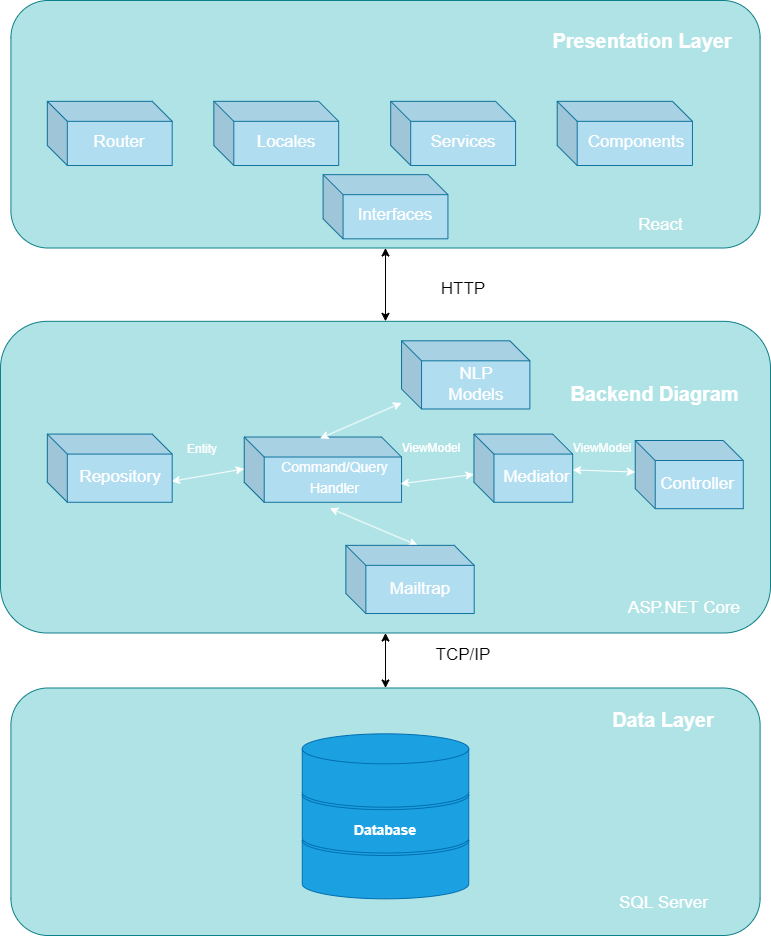
\includegraphics[height=200mm]{figs/conceptualArchitecture.png}
	\caption{Arhitectura conceptuală a sistemului}
	\label{fig:conceptualArchitecture}
\end{figure}
\newpage

\section{Structura bazei de date}
În figura \ref{fig:dbDiagram} este reprezentată diagrama bazei de date. Această diagramă a fost creată cu ajutorul dbdiagram.io~\cite{DbDiagram}
\begin{figure}[H]
	\centering
	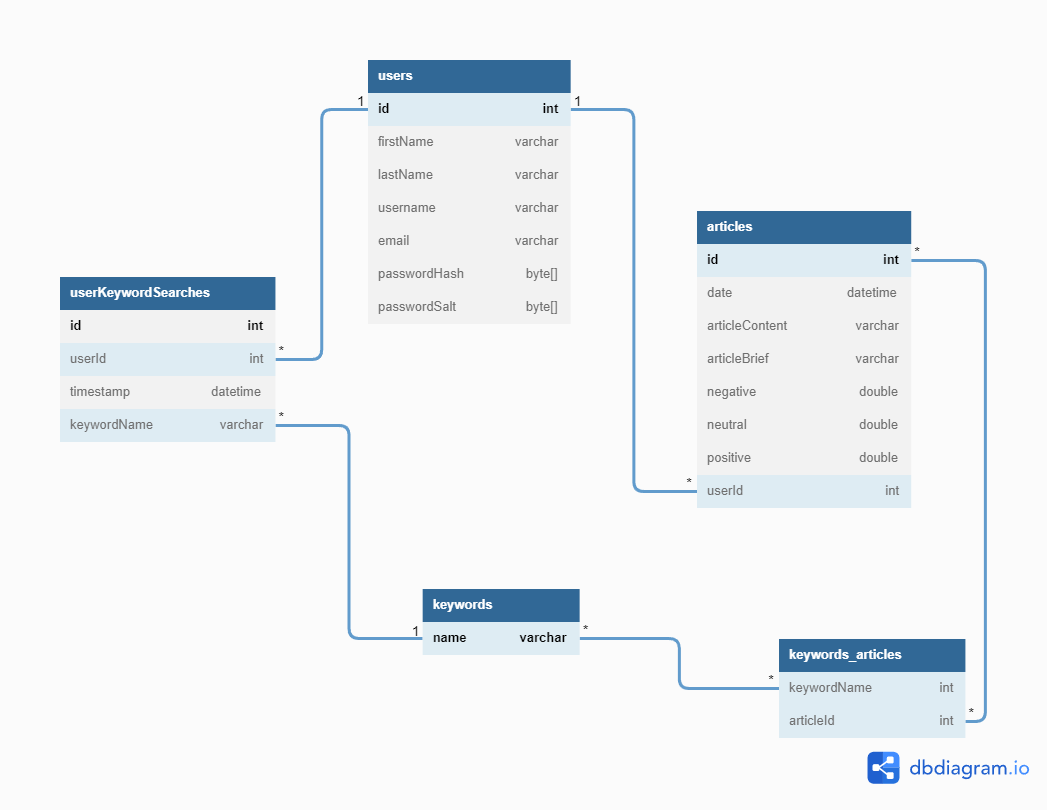
\includegraphics[width=150mm]{figs/dbDiagram.png}
	\caption{Diagrama bazei de date}
	\label{fig:dbDiagram}
\end{figure}

Tabelele din baza de date sunt următoarele: Users, Keywords, UserKeywordSearches, Articles și o tabelă pentru a ilustra relația dintre Keywords și Articles.
\subsubsection{Tabela Users}
Această tabelă conține informațiile despre un utilizator.
\begin{itemize}
	\setlength\itemsep{0.5em}
	\item Id - reprezintă Id-ul utilizatorului, un identificator unic și este cheie primară în acest tabel
	\item FirstName - reprezintă prenumele utilizatorului, nu poate fi null și nu include caractere speciale sau cifre
	\item LastName - reprezintă numele utilizatorului, nu poate fi null și nu include caractere speciale sau cifre
	\item Email - reprezintă email-ul utilizatorului, nu poate avea duplicat, trebuie să aiba formatul corect pentru email
	\item Username - reprezintă numele de utilizator, nu poate fi null, poate avea caractere speciale sau cifre
	\item PasswordHash și PasswordSalt - reprezintă parola utilizatorului (explicată în partea de nivel de aplicație), nu poate fi null
\end{itemize}

\subsubsection{Tabela Keywords}
Această tabelă conține informațiile despre un keyword.
\begin{itemize}
	\setlength\itemsep{0.5em}
	\item Name - reprezintă identificatorul keyword-ului (cuvântului cheie sau frazei) și este cheie primară în acest tabel
\end{itemize}

\subsubsection{Tabela UserKeywordSearches}
Această tabelă conține informațiile despre un cuvânt cheie sau expresie identificată în textul analizat de utilizator.
\begin{itemize}
	\setlength\itemsep{0.5em}
	\item UserId - reprezintă cheia străină în tabel, legătură cu utilizatorul care în a cărui analiză a fost identificat cuvântul cheie sau expresia
	\item Timestamp - reprezintă data când a fost efectuată analiza textului în care a fost identificat cuvântul cheie sau expresia
	\item KeywordName - reprezintă cheie străină în tabel, legătură cu cuvântul cheie sau expresia identificată în textul analizat de utilizator
\end{itemize}

\subsubsection{Tabela Articles}
Această tabelă conține informațiile despre un articol. În acest caz, articol reprezintă un rezultatul unei analize de text cu mai multe atribute care vor fi enumerate și explicate mai jos.
\begin{itemize}
	\setlength\itemsep{0.5em}
	\item Id - reprezintă Id-ul utilizatorului, un identificator unic și este cheie primară în acest tabel
	\item Date - reprezintă data când a fost salvat articolul (rezultatele obținute în urma analizei)
	\item ArticleContent - reprezintă conținutul inițial al textului, înainte de a fi efectuată analiza
	\item ArticleBrief - reprezintă conținutul sumarizat al textului, după ce a fost efectuată analiza
	\item Negative - reprezintă scorul negativ obținut în urma analizei de sentiment pe text financiar
	\item Neutral - reprezintă scorul neutru obținut în urma analizei de sentiment pe text financiar
	\item Positive - reprezintă scorul pozitiv obținut în urma analizei de sentiment pe text financiar
	\item UserId - reprezintă cheie străină în tabel, legătură cu utilizatorul care a analizat textul
\end{itemize}
\ \\
Relațiile între tabele sunt stabilite în felul următor: un utilizator poate realiza mai multe analize pe texte financiare, iar cuvintele cheie sau expresiile extrase reprezintă căutarile utilizatorului.
Deci un utilizator poate avea mai multe căutari, iar o căutare este legată de un singur utilizator.\\

\noindent Mai mult decât atât, în urma unei analize, utilizatorul poate salva rezultatele în istoricul său personal, creând o înregistrare nouă pentru un articol în baza de date. 
Un utilizator poate avea mai multe articole salvate, iar fiecare articol aparține unui utilizator. \\

\noindent Într-un articol sunt salvate cuvintele cheie sau expresiile identificate în urma analizei, așadar un articol poate avea mai multe cuvinte cheie și un cuvânt cheie poate fi identificat în mai multe articole, pentru diferiți utilizatori.\\

\section{Structura modulului de backend}
În figura \ref{fig:backendDiagram} este reprezentată diagrama modulului de backend.
\begin{figure}[H]
	\centering
	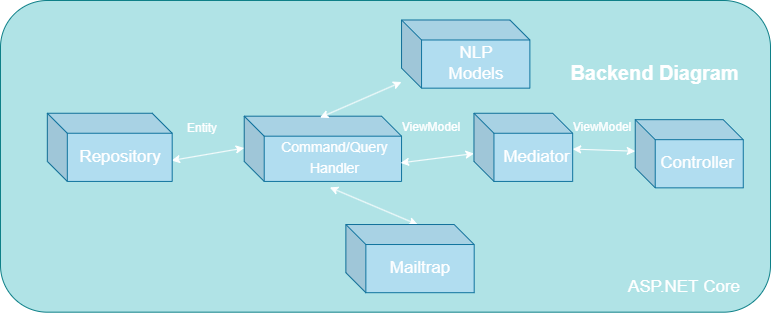
\includegraphics[width=150mm]{figs/backendDiagram.png}
	\caption{Diagrama modulului de backend}
	\label{fig:backendDiagram}
\end{figure}

Modulul de backend este, de fapt, serverul din arhitectura client-server. Acesta se ocupă de procesarea request-urilor venite de la utilizator folosind un mediator.\\
Problema pe care o rezolvă adăugarea unui mediator este decuplarea componentelor unui sistem. Acestea nu vor comunica în mod direct între ele, interacțiunea fiind mediată. Avantajul folosirii interacțiunii mijlocite 
constă în faptul că, dacă vor apărea modificări noi, componentele deja existente nu vor fi afectate. \\
Poate exista, într-adevăr, și un dezavantaj - poate ajunge destul de complex în funcție de cerințele sistemului, așa cum este menționat aici ~\cite{MediatorDisadvantage}.\\

Legătura dintre backend și baza de date se face în felul următor: în fișierul din modulul de backend există un fișier {\it appsettings.json} unde se declară un ConnectionString pentru conexiunea la baza de date (poate fi văzut în figura \ref{fig:connectionString}, creată utilizând~\cite{Carbon}). Acel string de conexiune conține numele
bazei de date și alte câteva atribute care permit conectarea, dar pot fi opționale. 

\begin{figure}[H]
	\centering
	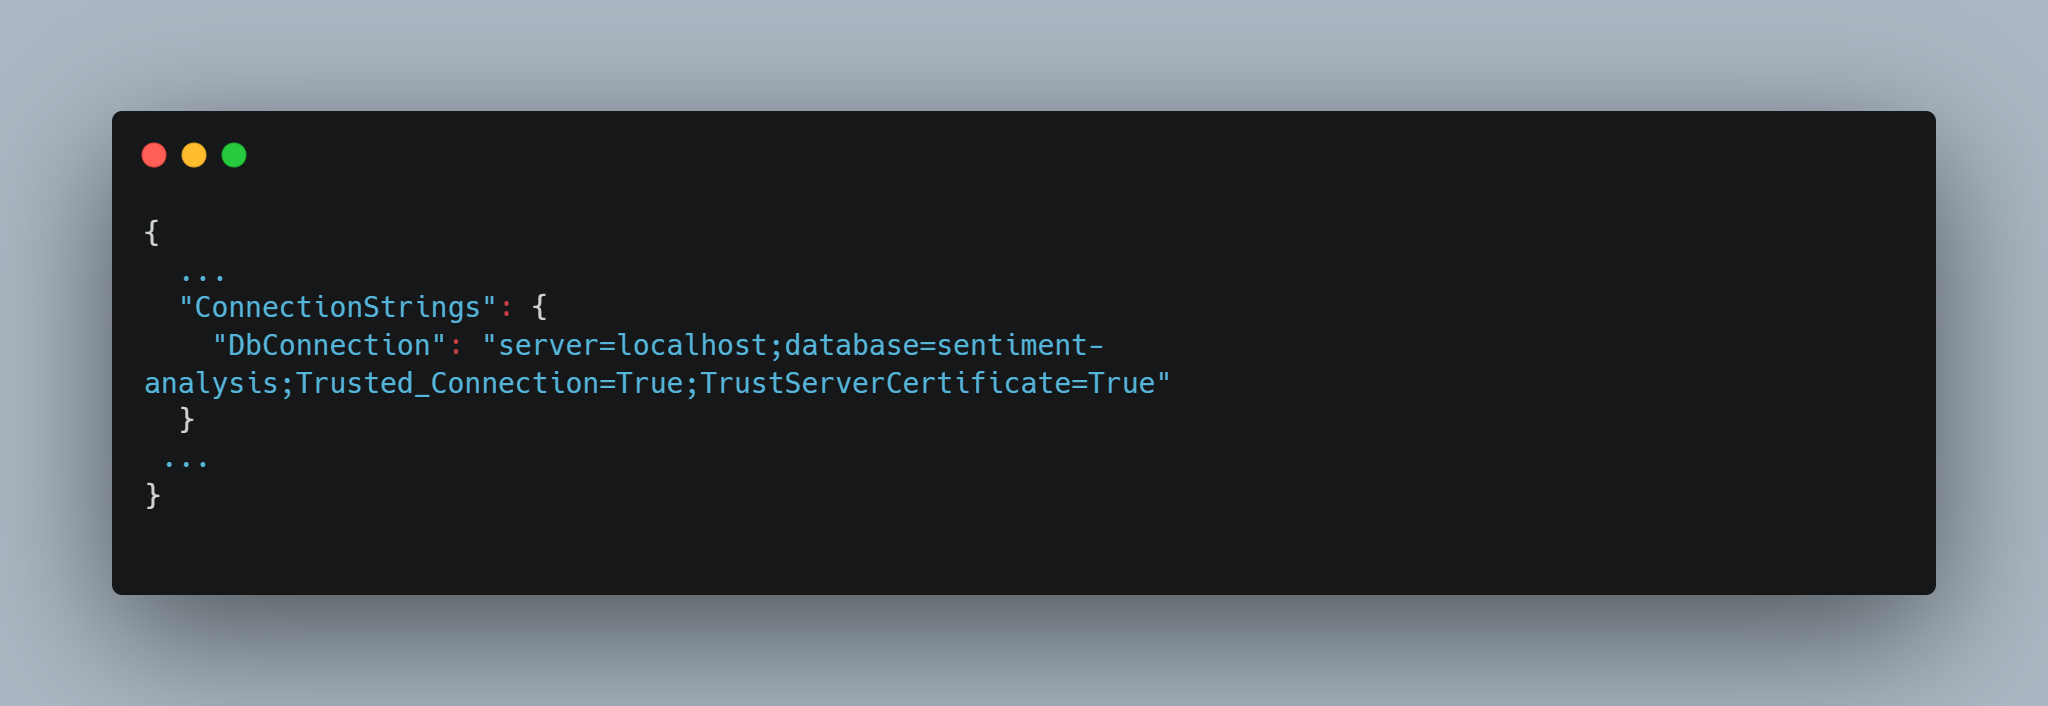
\includegraphics[width=150mm]{figs/connectionString.png}
	\caption{String de conectare backend cu baza de date}
	\label{fig:connectionString}
\end{figure}

\subsubsection{Repository}
În acest nivel se află legătura dintre aplicație și baza de date. Modelele create aici vor deveni entitați ale bazei de date.
Spre exemplu, clasa User cu atributele Id, FirstName, LastName, Username, Email, PasswordSalt, PasswordHash, va determina structura și atributele tabelei Users din baza de date, cea din urmă având toate atributele prezentate în clasă.

După crearea unui model, Entity Framework Core permite configurarea suplimentară a modelului, după cum poate fi văzut în figura \ref{fig:userEntityTypeConfiguration} și nu mai sunt necesare adnotări pentru atribute. În acest mod, a fost specificat că 
atributul de Id este cheie primară (implicit nu poate fi null), iar celelalte atribute FirstName, LastName, Username, Email, PasswordHash, PasswordSalt trebuie să fie diferite de null. 
\begin{figure}[H]
	\centering
	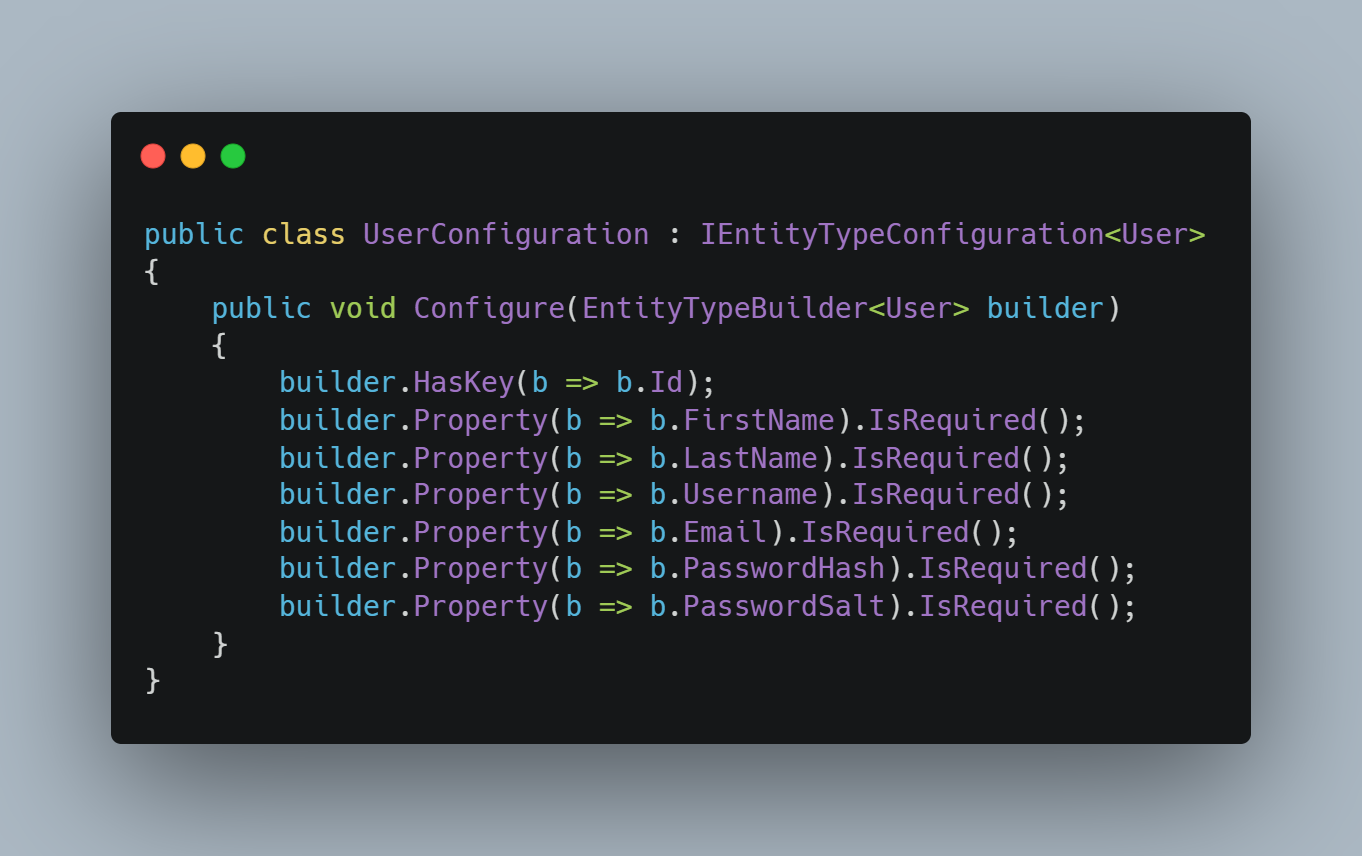
\includegraphics[width=100mm]{figs/userEntityTypeConfiguration.png}
	\caption{Configurare pentru modelul unui utilizator}
	\label{fig:userEntityTypeConfiguration}
\end{figure}

Aici se introduce conceptul de DbContext, care reprezintă o sesiune cu baza de date, când se pot face operații de tip stocare, interogare, actualizare și ștergere a elementelor din baza de date, creare de modele și maparea datelor.\\
DbContext este responsabil de deschiderea și gestionarea conexiunilor cu baza de date. \\
Pentru crearea unui model, DbContext îl construiește bazându-se pe configurarea dată și apoi este mapat. Pentru maparea datelor, rezultatele interogărilor sunt mapate la instanțe și entități definite de utilizator, cum sunt in figura \ref{fig:dbContext}.\\

Se adaugă conceptul de DbSet, prin care este posibilă aplicarea operațiilor de tip stocare, interogare, actualizare, ștergere pe acea entitate.\\
Clasele DbSet sunt proprietăți ale DbContextului și sunt mapate la baza de date care iau numele dat de utilizator.
DbSet este o implementare a patternului Repository, care înceară să adauge un layer între nivelul de acces la baza de date și nivelul de logică.

\begin{figure}[H]
	\centering
	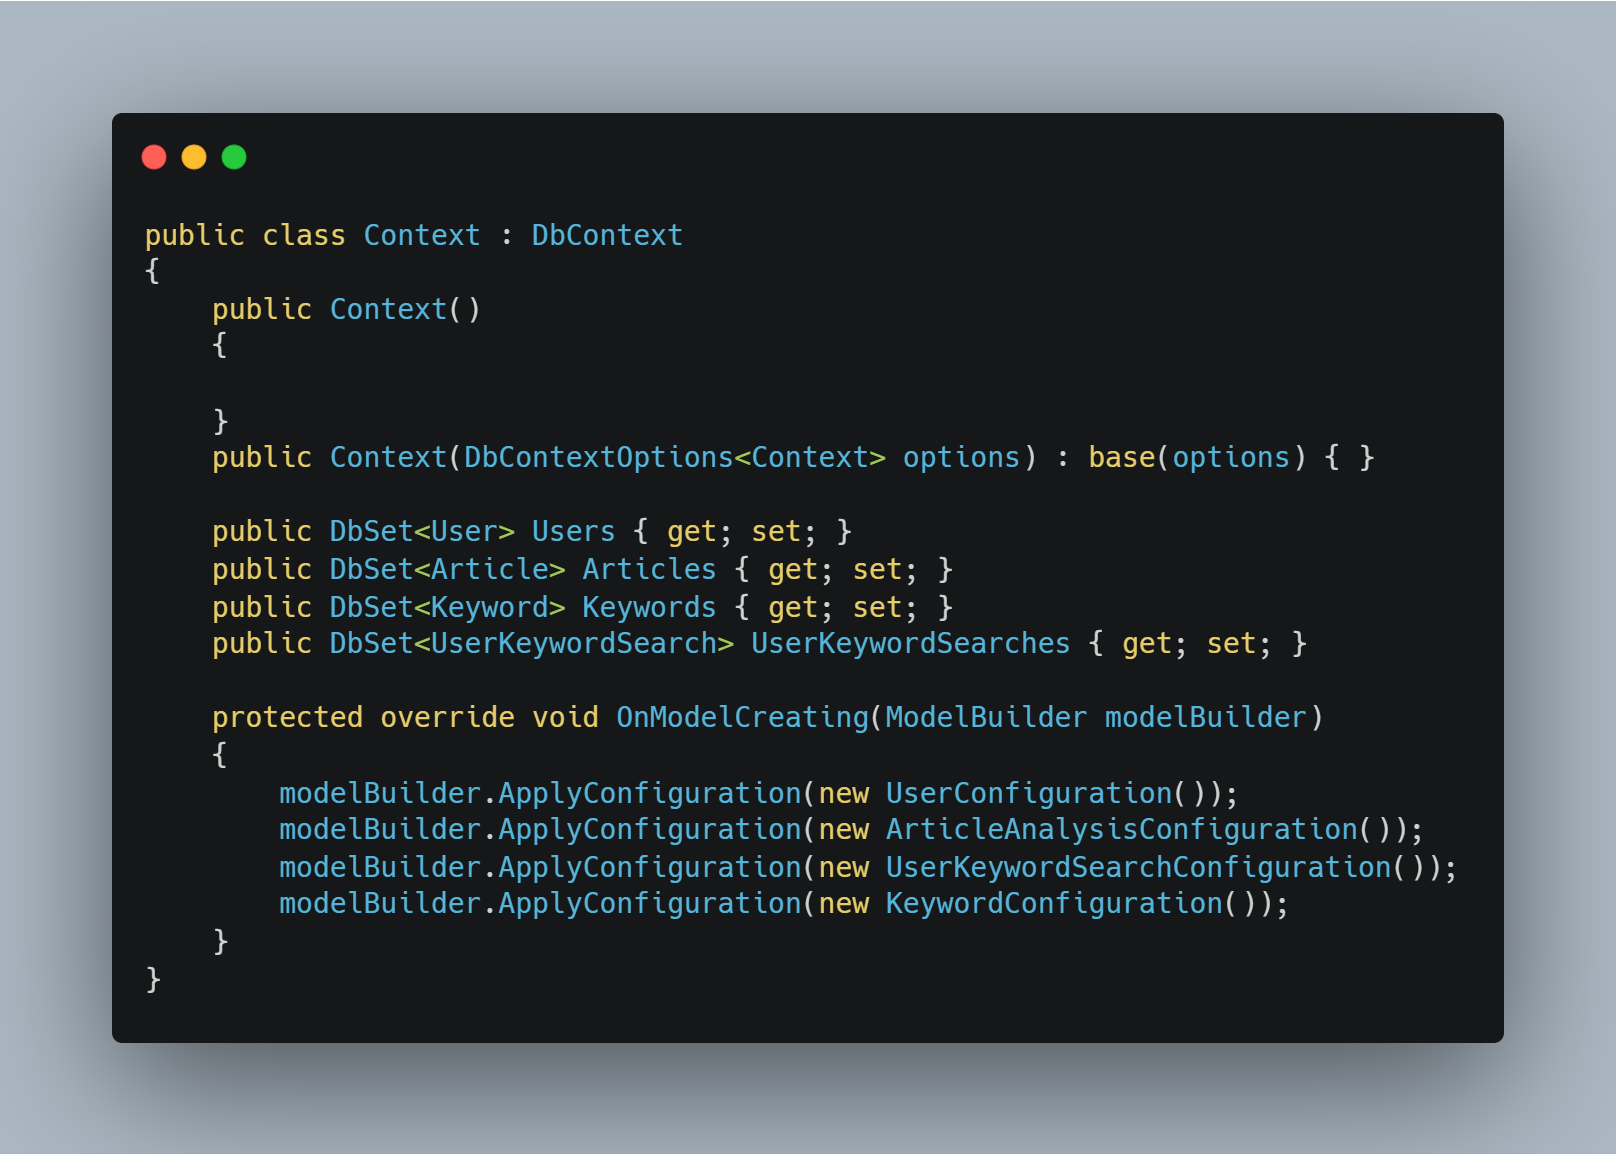
\includegraphics[width=150mm]{figs/dbContext.png}
	\caption{Configurare DbContext}
	\label{fig:dbContext}
\end{figure}

\subsubsection{Command/Query Handler}
Aici se află partea de logică și procesare a datelor din aplicație. Prin procesarea datelor înțelegem toate interacțiunile ce pot exista cu baza de date și din această cauză a fost introdus un pattern al cărui scop este de separare a operațiilor de citire și scriere în baza de date - CQRS sau Command and Query Responsibility Segregation. \\

Așadar, se face o separare în 2 modele, comenzi și interogări. Comenzile sunt, de fapt, operațiile ce presupun stocarea, actualizarea sau ștergerea din baza de date, iar interogările reprezintă citirile din baza de date. \\
În partea de comenzi, operațiile care se fac sunt următoarele, în funcție de clasă:
\begin{itemize}
	\setlength\itemsep{0.5em}
	\item User
	\begin{itemize}
		\setlength\itemsep{0.5em}
		\item AddUserCommand - care adaugă un utilizator nou, folosită pentru crearea unui cont nou
		\item EditUserCommand - care actualizează detaliile unui utilizator
		\item DeleteUserCommand - care șterge un utilizator
	\end{itemize}
	\item UserKeywordSearches
	\begin{itemize}
		\setlength\itemsep{0.5em}
		\item AddUserKeywordSearchCommand - care adaugă o nouă căutare ce cuprinde cuvântul cheie sau expresia identificată în textul analizat
	\end{itemize}
	\item Articles
	\begin{itemize}
		\setlength\itemsep{0.5em}
		\item AddArticleCommand - care adaugă un nou articol ce cuprinde toate rezultatele analizei efectuate pe un text financiar
		\item DeleteArticleCommand - care șterge un articol ce cuprinde toate rezultatele analizei efectuate pe un text financiar
	\end{itemize}
\end{itemize}
În partea de interogări, operațiile care se fac sunt următoarele, în funcție de clasă:
\begin{itemize}
	\setlength\itemsep{0.5em}
	\item User
	\begin{itemize}
		\setlength\itemsep{0.5em}
		\item GetUserDetailsQuery - care cere informațiile despre un anumit utilizator, într-un anumit format solicitat
		\item EditUserCommand - care actualizează detaliile unui utilizator
		\item DeleteUserCommand - care șterge un utilizator
	\end{itemize}
	\item UserKeywordSearches
	\begin{itemize}
		\setlength\itemsep{0.5em}
		\item GetKeywordStatisticsQuery - care interoghează baza de date și trimite înregistrările găsite pentru un anumit cuvânt cheie sau expresie într-o perioadă selectată
		\item GetSearchNumberOfOccurrencesQuery - care interoghează baza de date și trimite înregistrările pe zile pentru itemii (cuvinte cheie sau expresii) găsite în perioada selectată de timp
		\item FilterSearchesByPeriodCommand - care interoghează baza de date și trimite înregistrările găsite într-o perioadă selectată pentru cele mai populare 10 subiecte
	\end{itemize}
	\item Articles
	\begin{itemize}
		\setlength\itemsep{0.5em}
		\item GetArticlesQuery - care interoghează baza de date și trimite înregistrările găsite pentru pentru un anumit input, adică toate articolele salvate ale unui utilizator
		\item GetUserArticleQuery - care interoghează baza de date și trimite informații despre articolul selectat pentru ca utilizatorul să poată revedea analiza detaliată
	\end{itemize}
	\item TextAnalysis
	\begin{itemize}
		\setlength\itemsep{0.5em}
		\item GetSentimentScoreQuery - care realizează inferența modului de analiză de sentiment având drept input textul introdus de utilizator
		\item GetTextSummaryQuery -  care realizează inferența modului de sumarizare a textului având drept input textul introdus de utilizator
		\item GetKeyphrasesQuery - care realizează inferența modului de extragere a cuvintelor cheie sau expresiilor având drept input textul introdus de utilizator
	\end{itemize}
\end{itemize}
\paragraph{Model de comandă}
\begin{figure}[H]
	\centering
	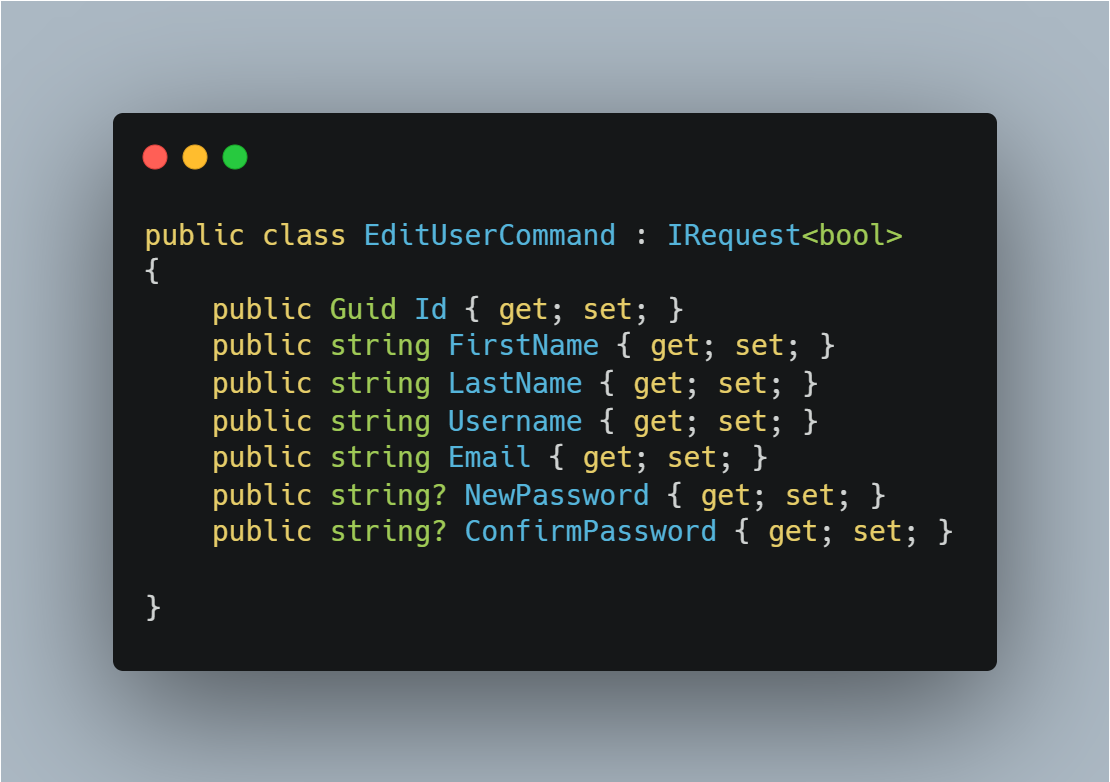
\includegraphics[width=100mm]{figs/editUserCommand.png}
	\caption{Comandă de editare utilizator}
	\label{fig:editUserCommand}
\end{figure}
Interfața IRequest acceptă tipul obiectului pe care Handlerul ar trebui să îl returneze, în acest caz, o valoare true sau false.
Un handler pentru această comandă este următorul, în figura \ref{fig:editUserCommandHandler}.
\begin{figure}[H]
	\centering
	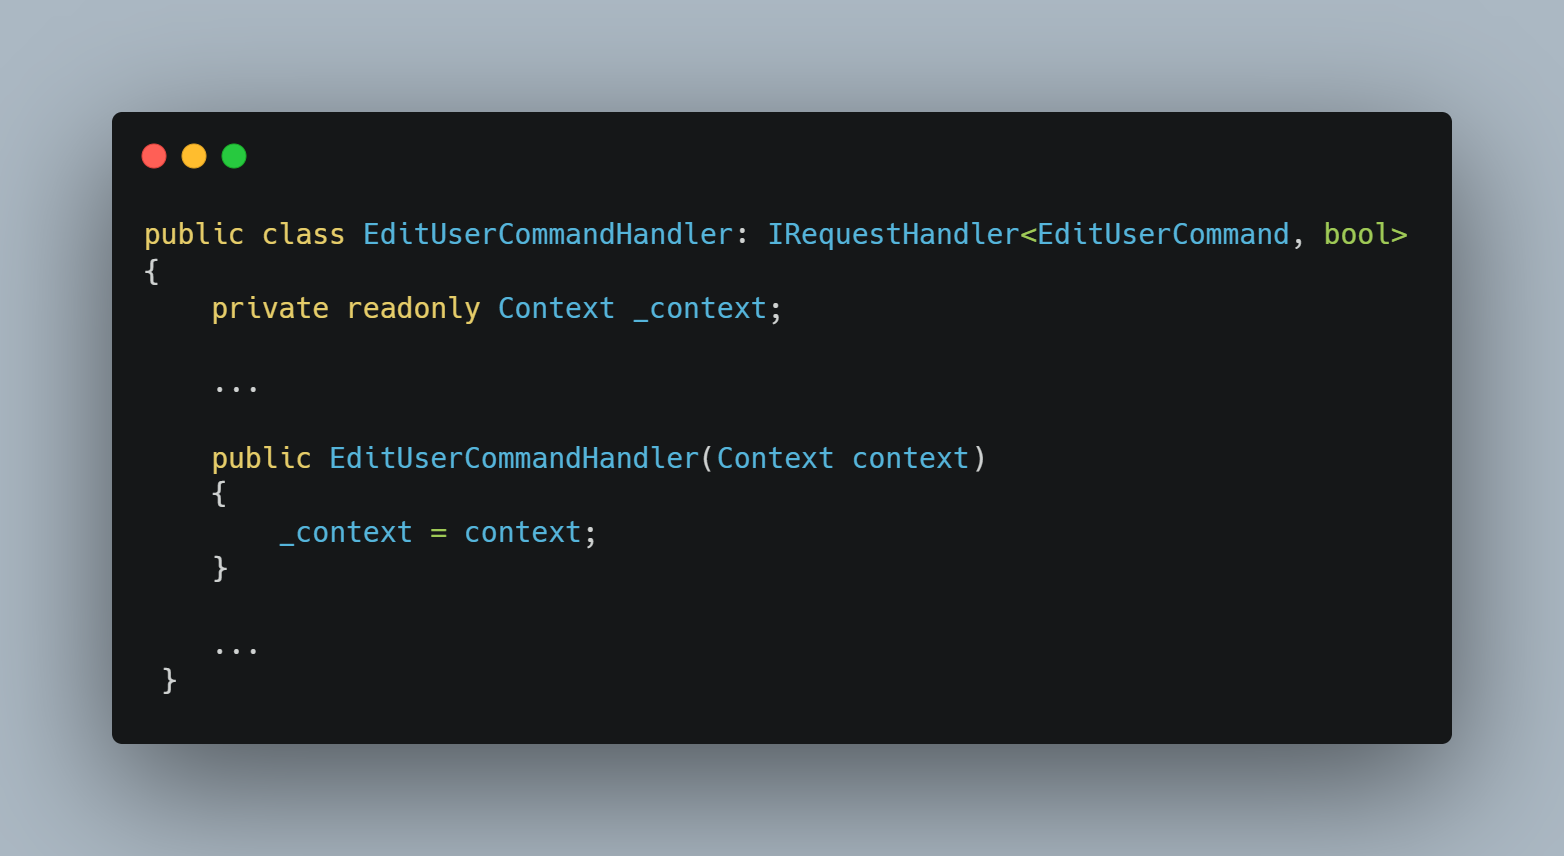
\includegraphics[width=150mm]{figs/editUserCommandHandler.png}
	\caption{Handler pentru comanda de editare utilizator}
	\label{fig:editUserCommandHandler}
\end{figure}
IRequestHandlerul acceptă 2 tipuri de parametri, după cum e specificat și aici~\cite{IRequestHandler}: requestul la care trebuie să răspundă și tipul care trebuie returnat.
\paragraph{Model de query}
În figura \ref{fig:getUserArticleQuery} este un query care solicită ca răspuns un ArticleViewModel (un model pentru vizualizare a unui articol salvat de utilizator), atunci când primește ca identificatori un UserId și un ArticleId.
Handlerul poate fi văzut în figura \ref{fig:getUserArticleQueryHandler}.
\begin{figure}[H]
	\centering
	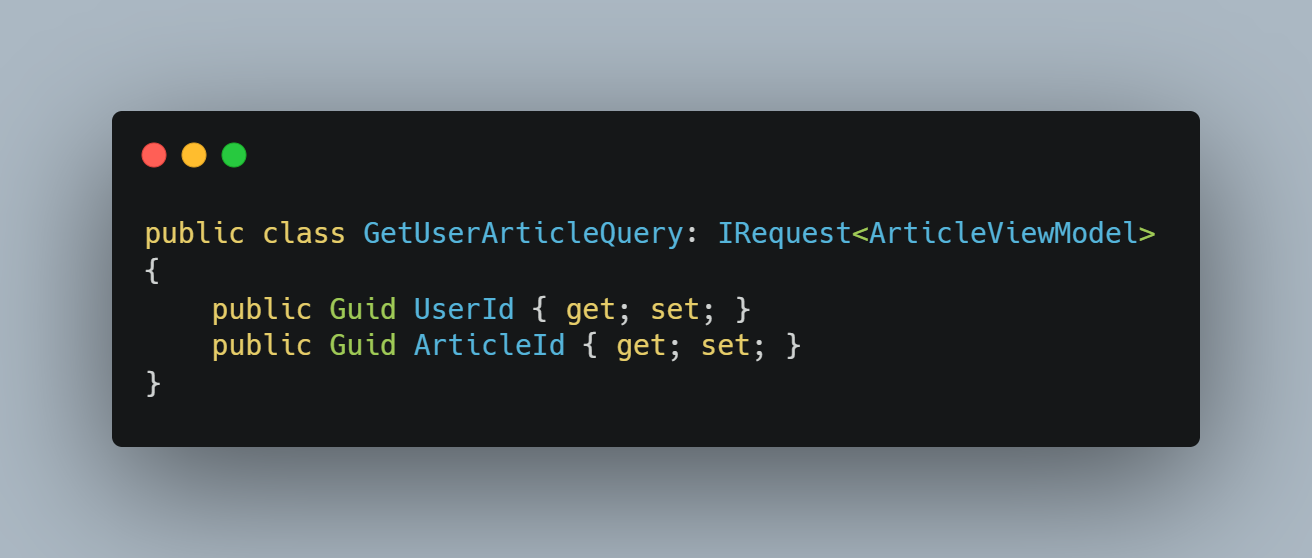
\includegraphics[width=100mm]{figs/getUserArticleQuery.png}
	\caption{Query de citire a informațiilor despre un articol salvat de utilizator}
	\label{fig:getUserArticleQuery}
\end{figure}

\begin{figure}[H]
	\centering
	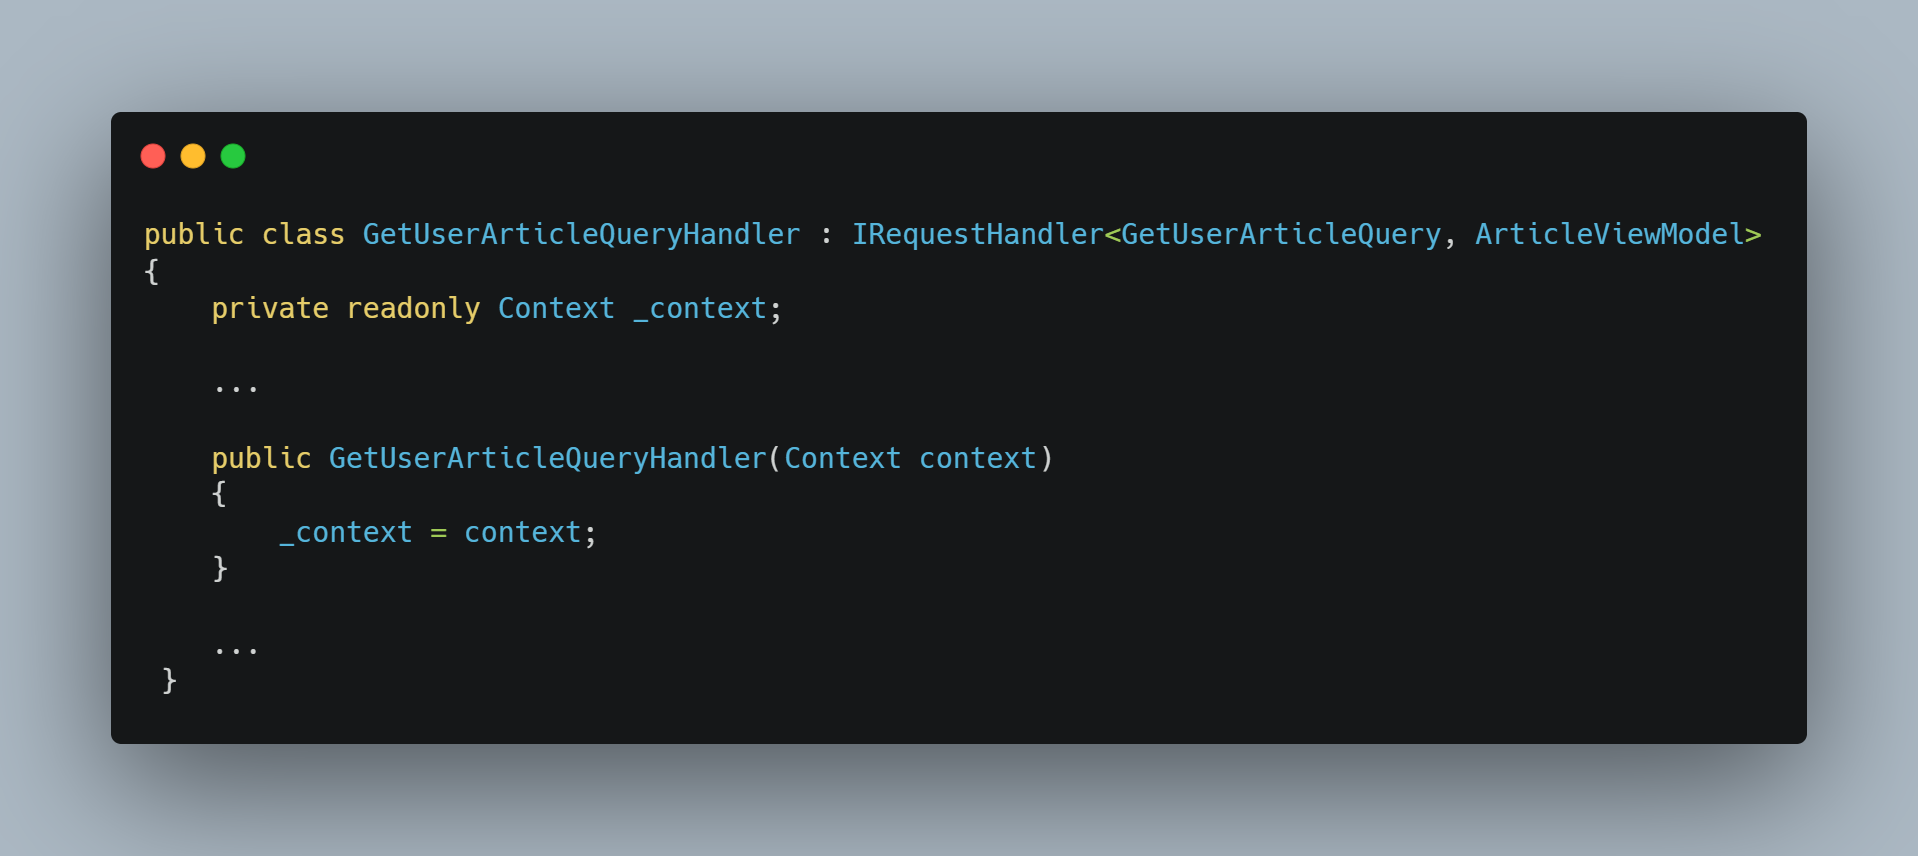
\includegraphics[width=100mm]{figs/getUserArticleQueryHandler.png}
	\caption{Handler al unui query de citire a informațiilor despre un articol salvat de utilizator}
	\label{fig:getUserArticleQueryHandler}
\end{figure}

\begin{figure}[H]
	\centering
	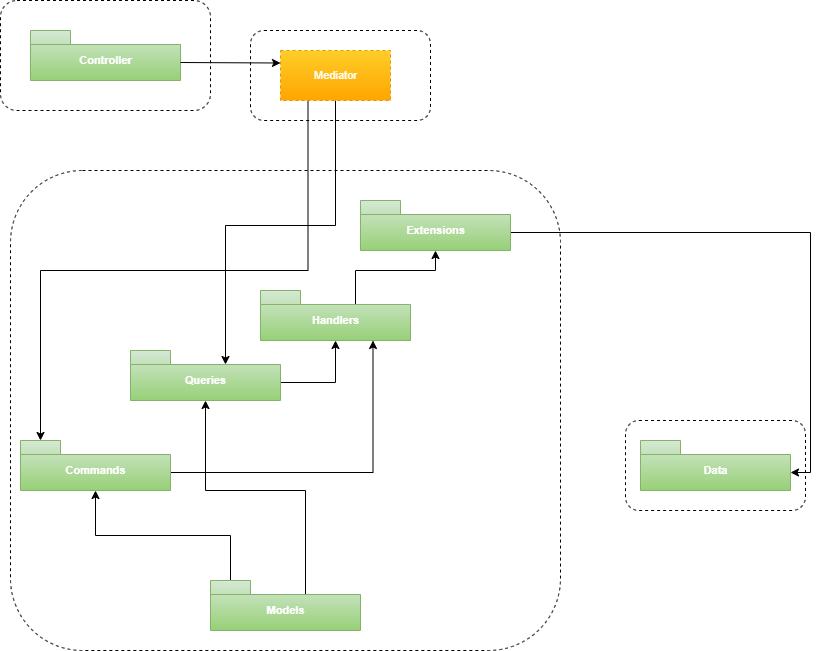
\includegraphics[width=150mm, height=100mm]{figs/packageBE.png}
	\caption{Diagrama pachetelor din modulul de backend}
	\label{fig:packageBE}
\end{figure}

După cum se poate vedea, handlerul este asemănător cu handler-ul comenzii de mai sus, diferența o face rezultatul trimis și metodele de validare din clase.
Tot în partea de logică a aplicației, sunt câteva handlere cu funcționalitate mai specială. 
\paragraph{Adăugare user nou}
\ \\
La crearea unui cont nou, în comandă sunt scrise toate informațiile necesare. De aici, câmpul de email mai este folosit și în trimiterea unui mail de confirmare a înregistrării. 
Pentru acest lucru am folosit Mailtrap, un server SMTP care ajută la testarea acestei funcționalități. 
Handlerul pentru această funcționalitate este în figura \ref{fig:sendRegistrationMail}.
\begin{figure}[H]
	\centering
	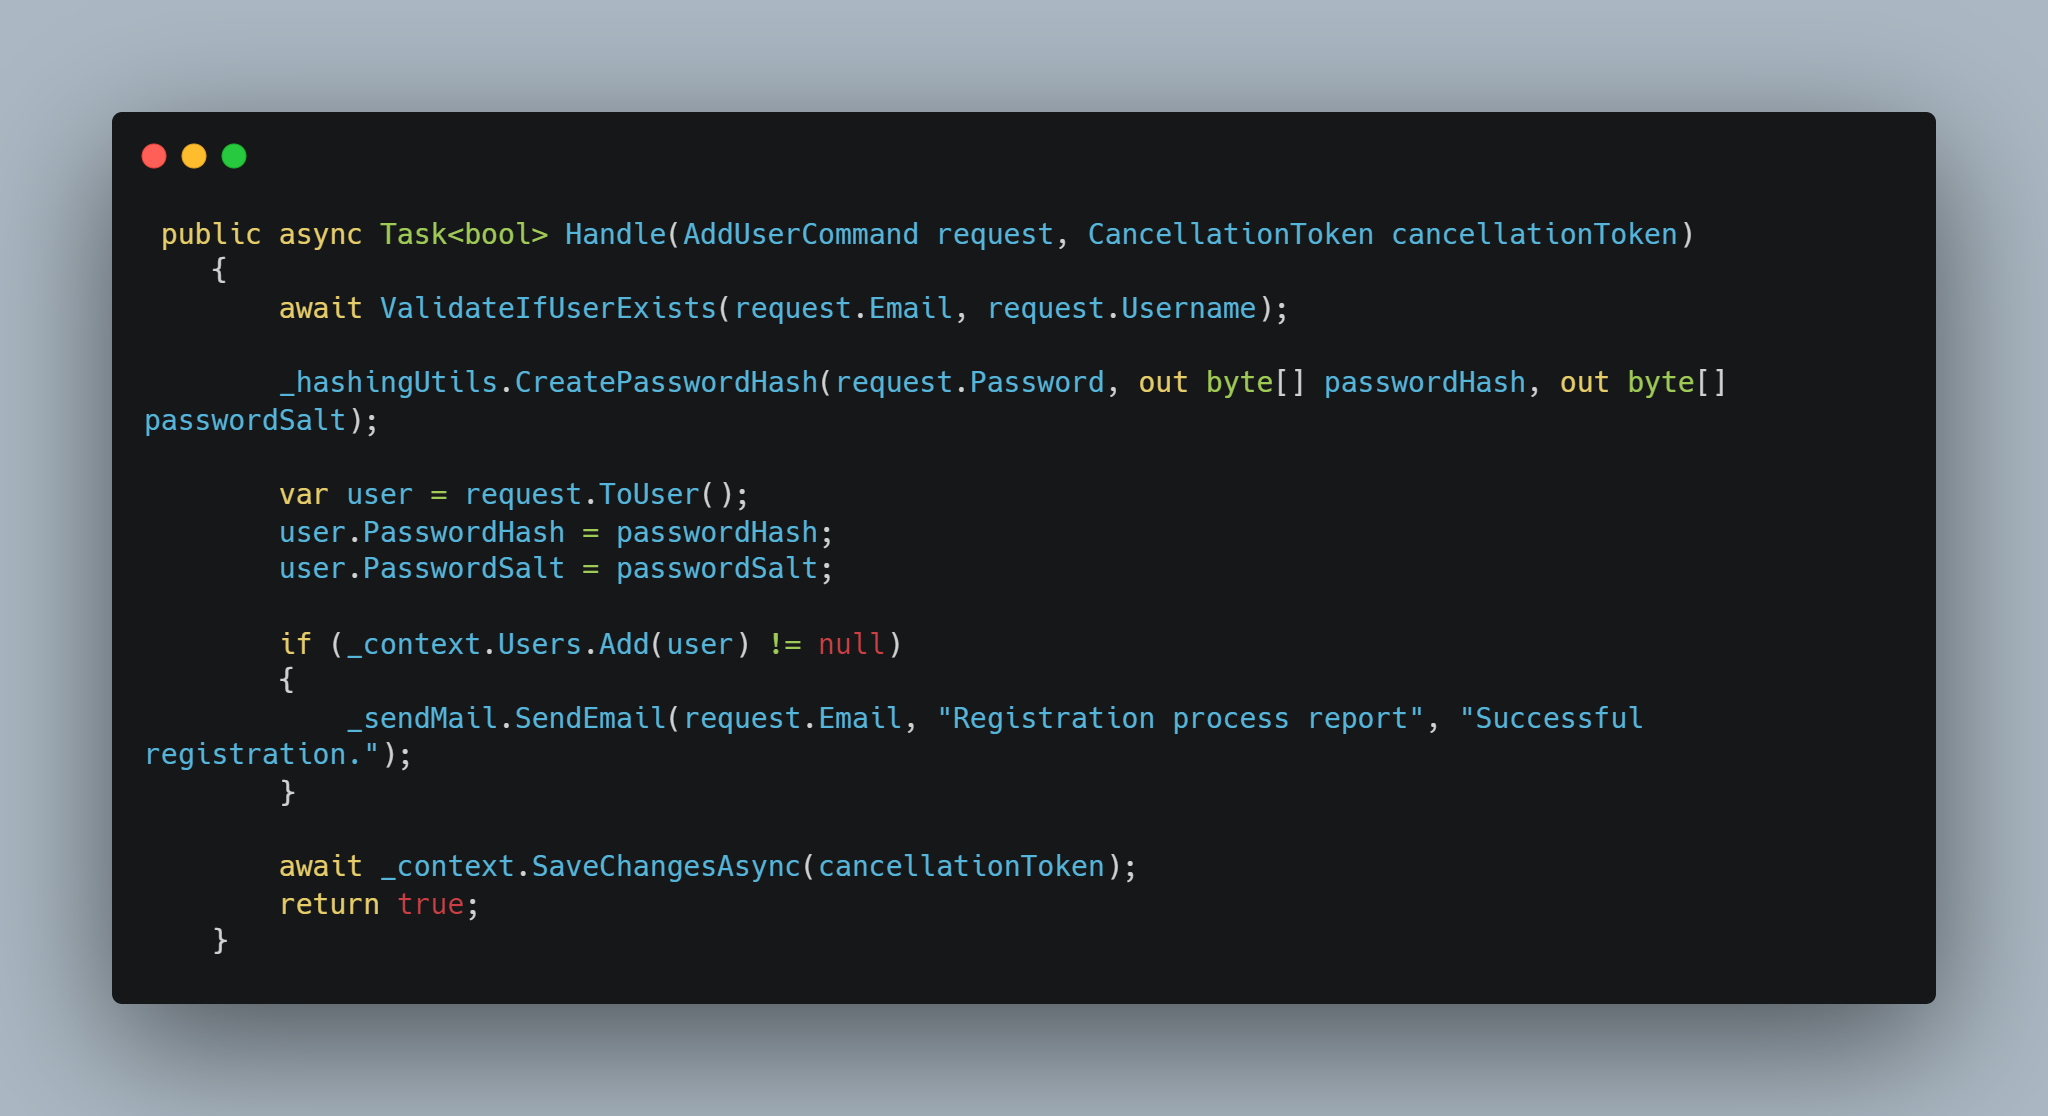
\includegraphics[width=100mm]{figs/sendRegistrationMail.png}
	\caption{Handler al unui query de citire a informațiilor despre un articol salvat de utilizator}
	\label{fig:sendRegistrationMail}
\end{figure}
Mai întâi se verifică dacă mai există alt utilizator cu același email sau nume de utilizator. În cazul în care există, va fi aruncată o excepție, altfel se continuă cu crearea unei parole criptate, se adaugă noul utilizator în baza de date și se trimite un email. 
Un exemplu de email este în figura \ref{fig:registrationReport}.
\begin{figure}[H]
	\centering
	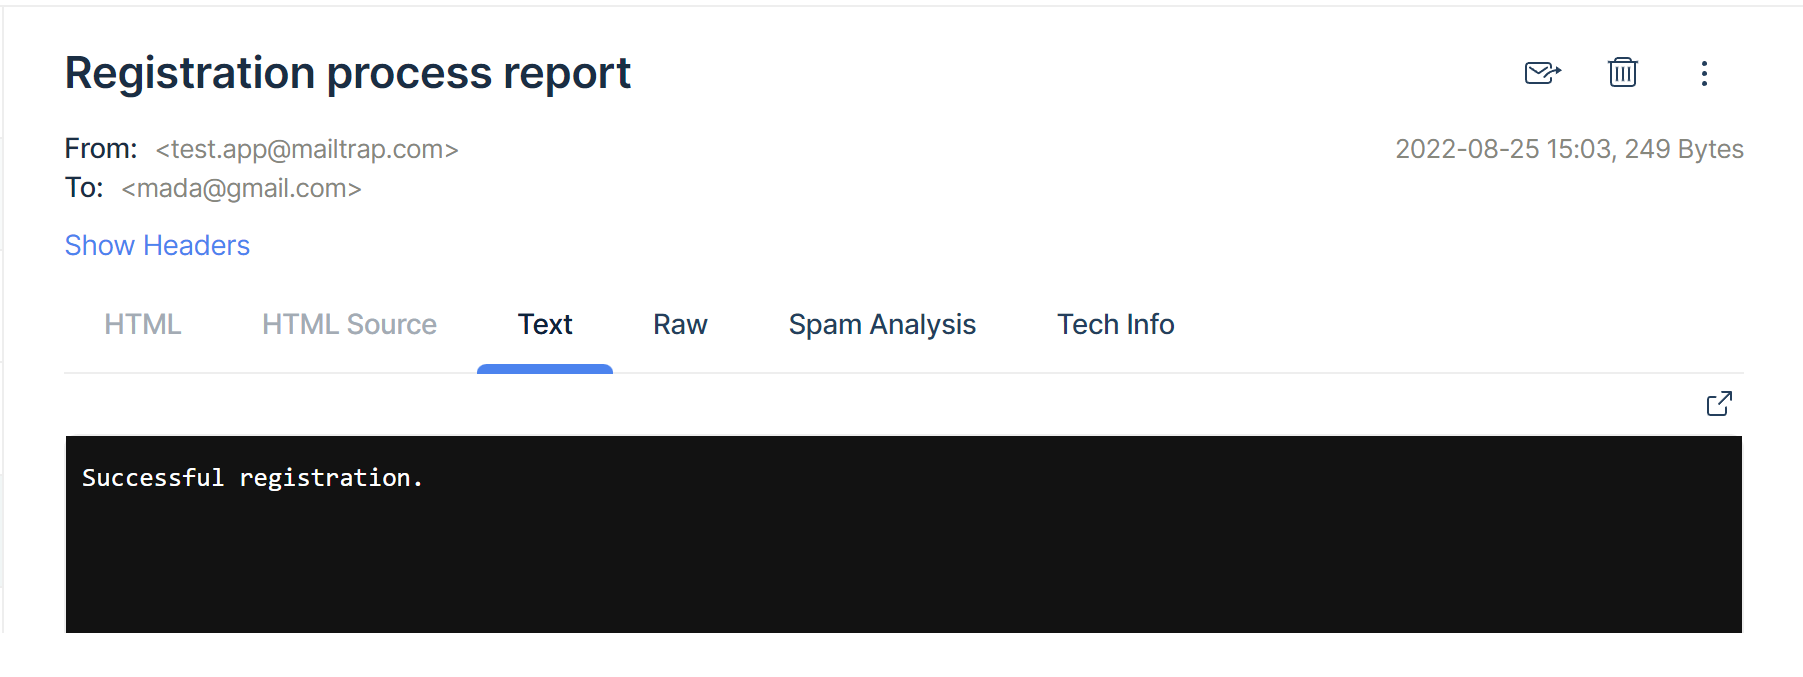
\includegraphics[width=100mm]{figs/registrationReport.png}
	\caption{Email de confirmare a procesului de creare de cont cu succes}
	\label{fig:registrationReport}
\end{figure}


Handlerele care se ocupă de analiza sentimentelor dintr-un text financiar, sumarizarea textului și extragerea cuvintelor cheie se află tot aici. Acestea folosesc un serviciu pentru a apela metodele specifice,exemplu în figururile \ref{fig:getKeyphrasesHelper} și \ref{fig:huggingFaceHelper} .
\begin{figure}[ht]
	\centering
	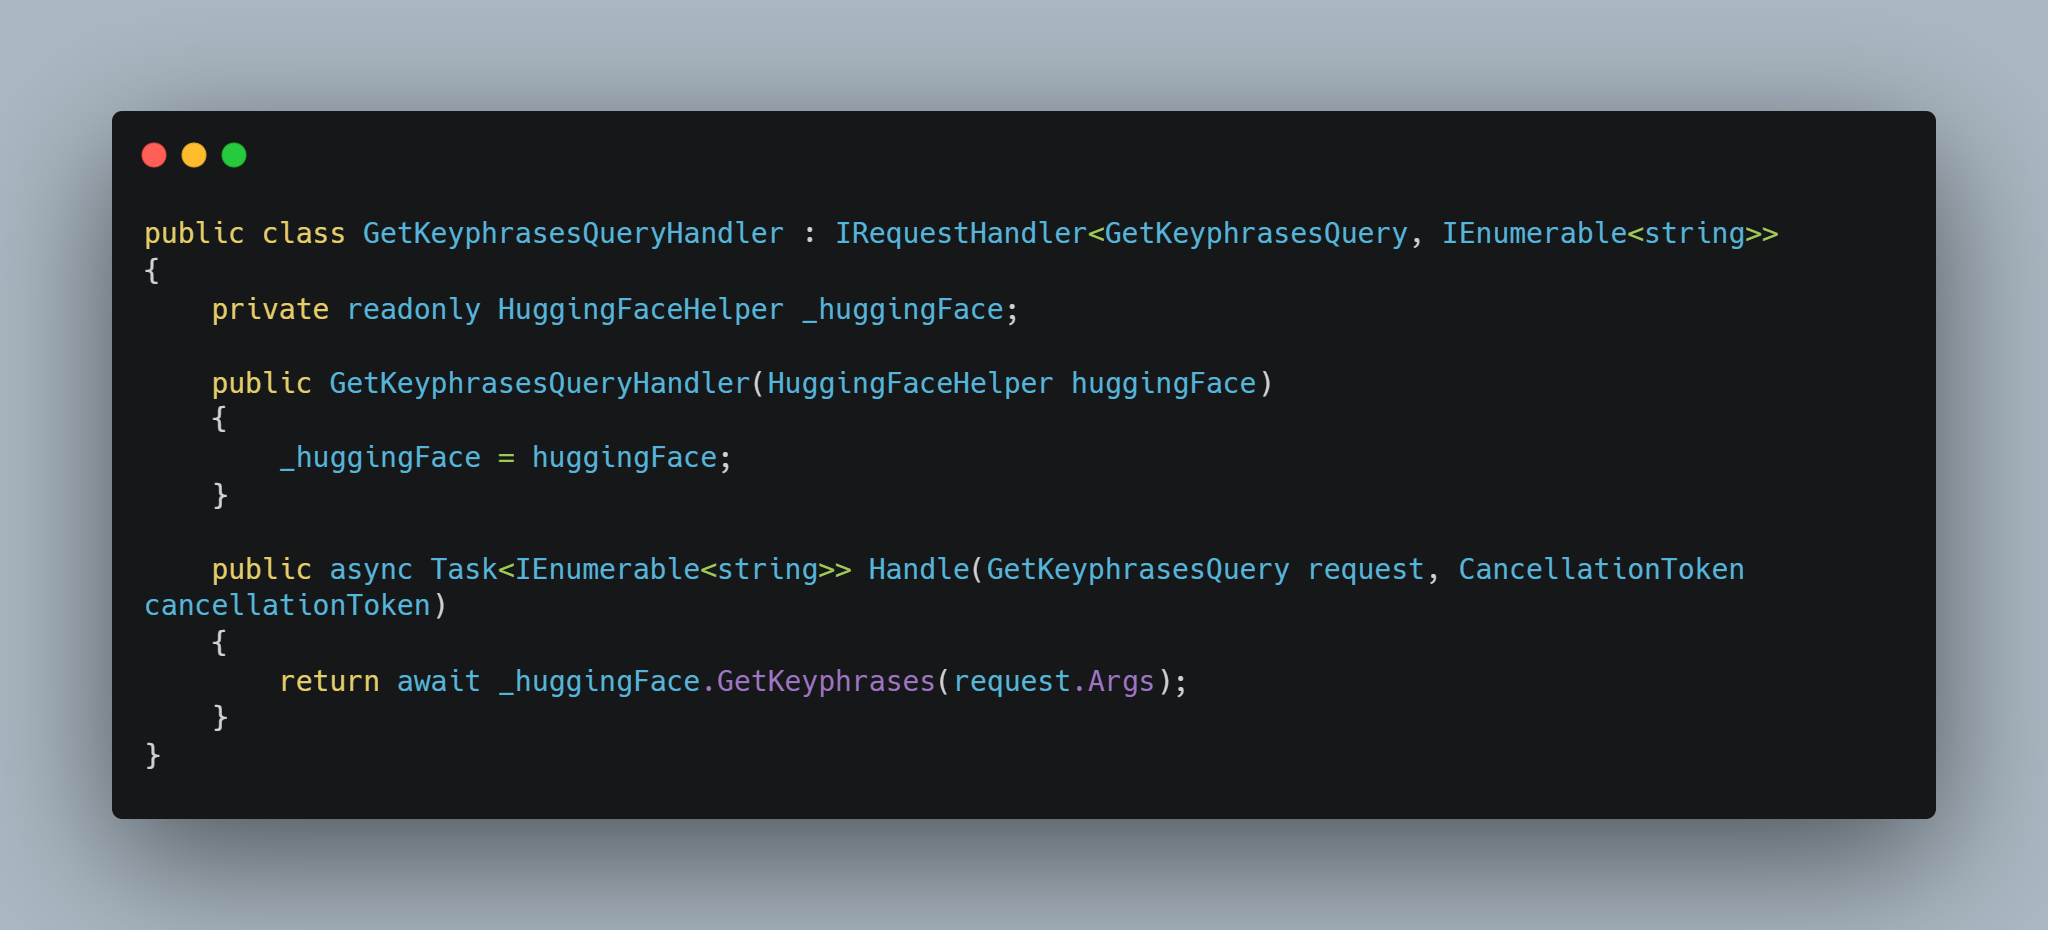
\includegraphics[width=150mm]{figs/getKeyphrasesHelper.png}
	\caption{Handler pentru extragerea cuvintelor cheie}
	\label{fig:getKeyphrasesHelper}
\end{figure}

Handlerul apelează metoda GetKeyphrases, având ca parametru textul introdus de utilizator. \\ HuggingFaceHelper este utilizat ca un serviciu și este posibilă apelarea metodelor din clasă. \\
Metoda menționată apelează altă metodă, CallModel, cu un URL pentru modelul care extrage cuvintele cheie și inputul utilizatorului. În această metodă, se creează un body în format JSON pentru un request de tip POST,
se trimite, apoi se așteaptă răspunsul. \\ 

Dacă răspunsul nu conține mesaj de eroare, acesta este transmis spre client, altfel se face o extra-validare pentru a detecta dacă eroarea primită este o eroare din cauza încărcării modelului, iar în cazul care este,
metoda se va apela recursiv pentru a porni modelul și a primi rezultatul așteptat, după ce vor mai fi efectuate câteva parsări pentru formatul corect al acestuia. 

\begin{figure}[ht]
	\centering
	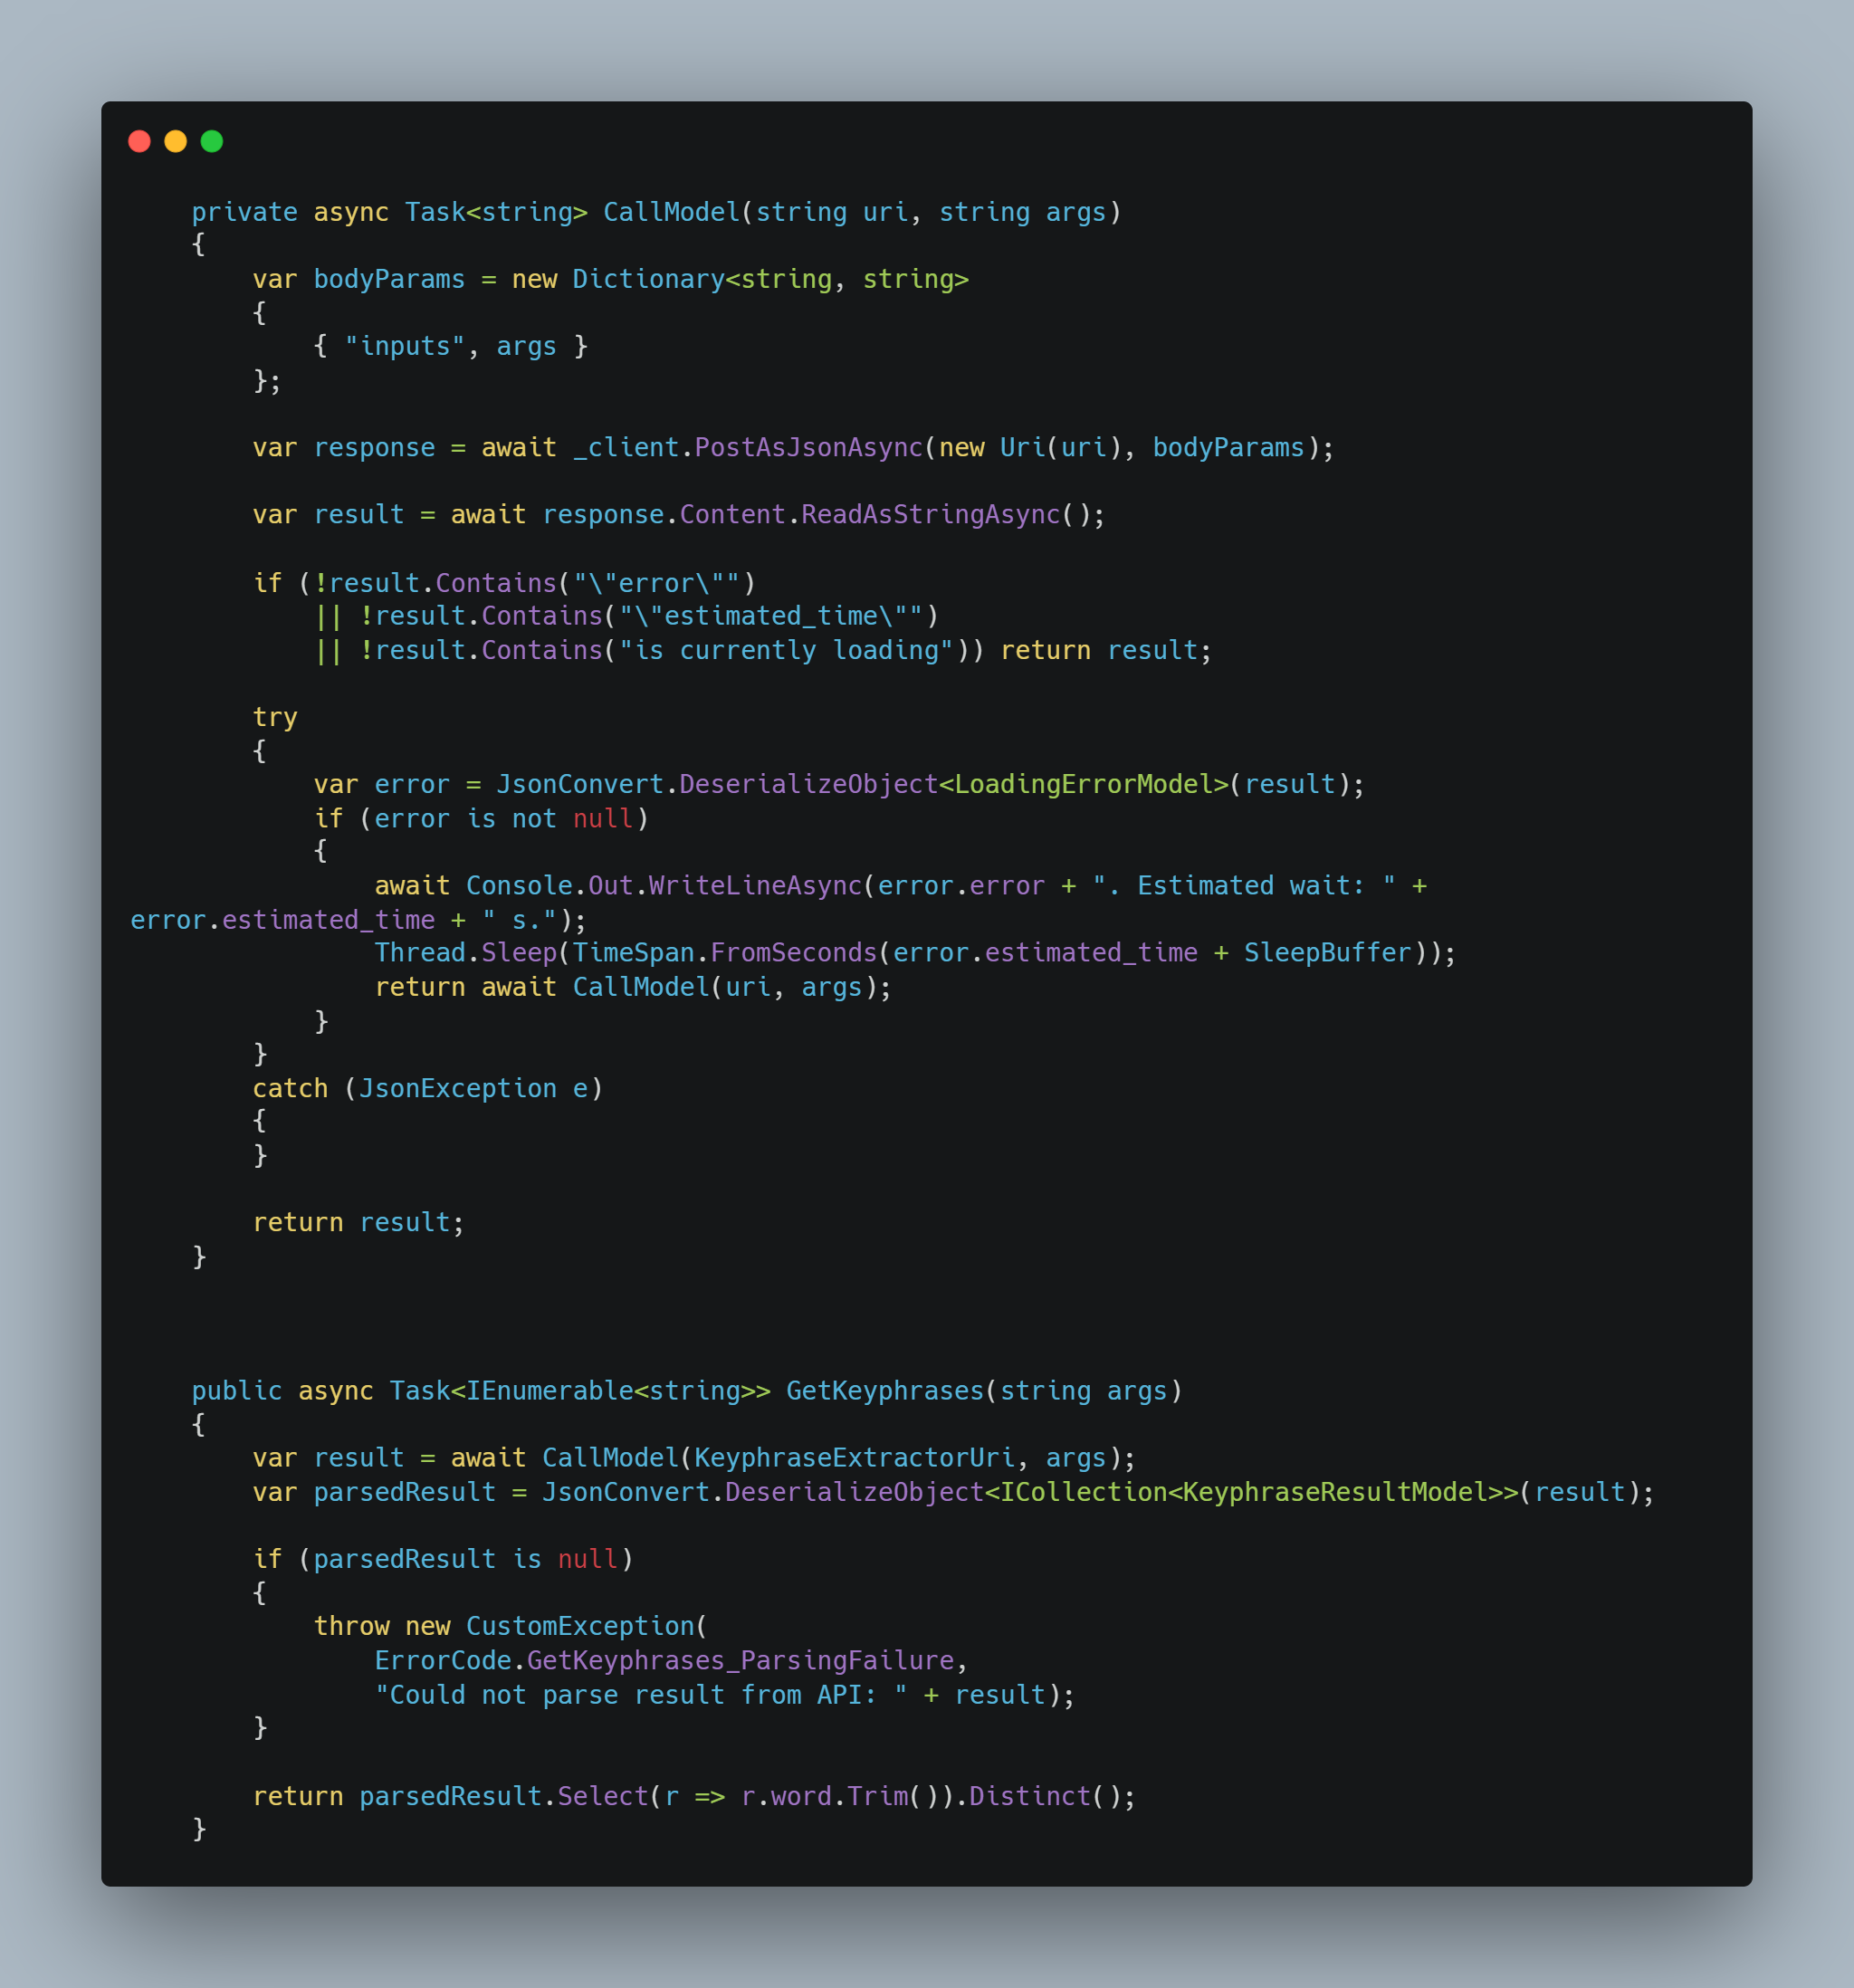
\includegraphics[width=150mm]{figs/huggingFaceHelper.png}
	\caption{Metode pentru a accesa funcționalitățile modelului NLP}
	\label{fig:huggingFaceHelper}
\end{figure}

Pentru cazurile în care metodele de validare aruncă excepții, pentru claritate cât mai mare a fluxului, excepțiile au fost customizate cu scopul de a fi transmise în format JSON în frontend și pentru a ajuta utilizatorul.
\begin{figure}[H]
	\centering
	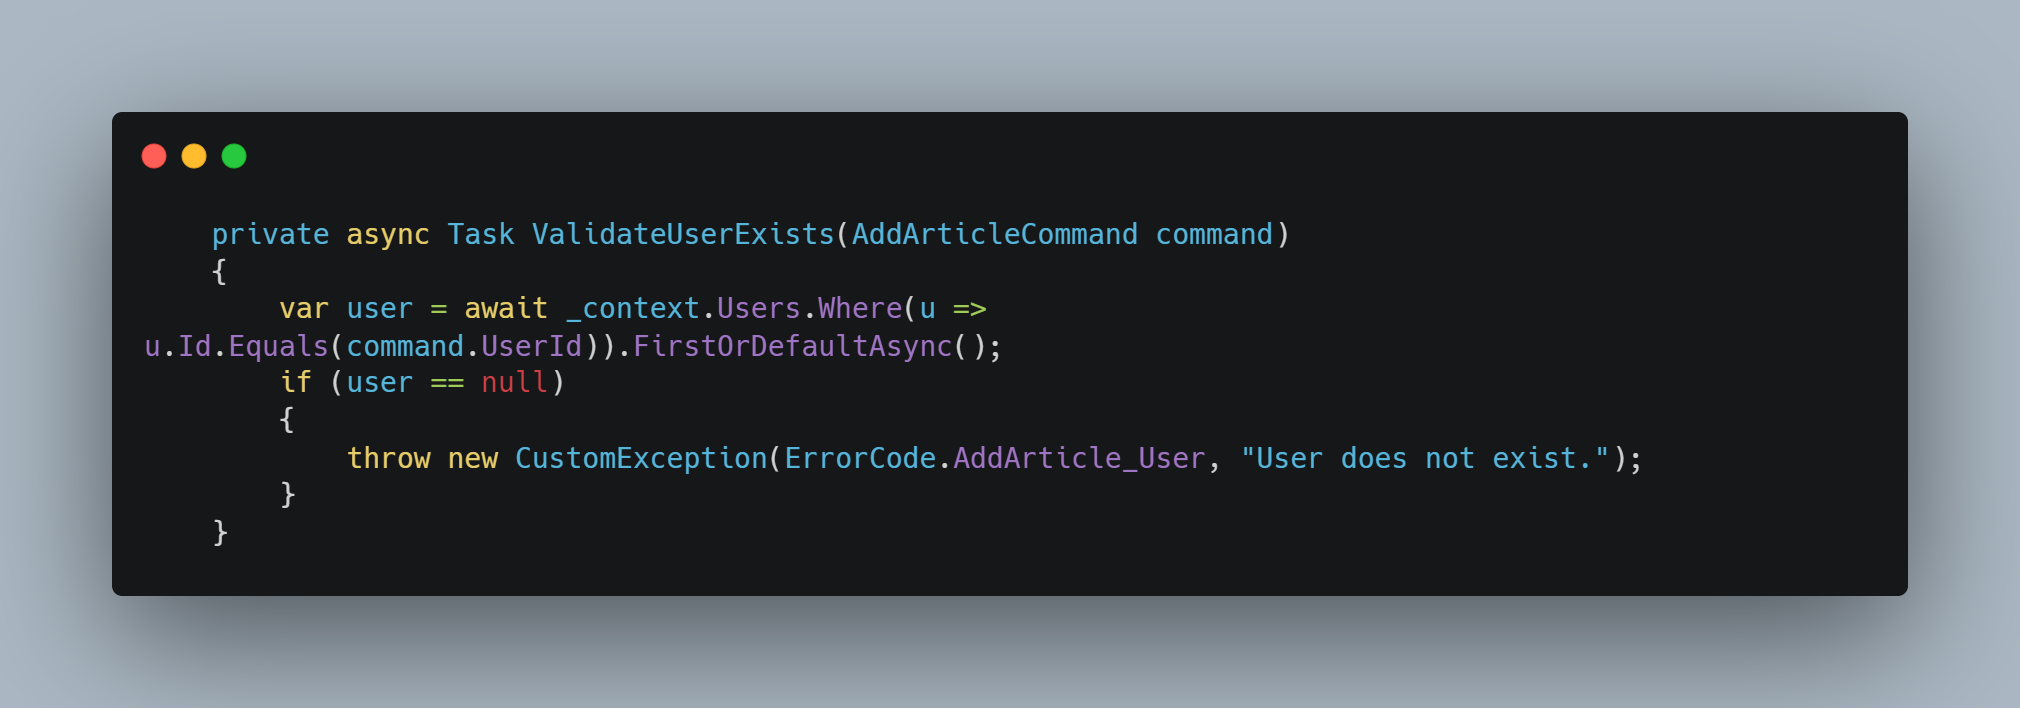
\includegraphics[width=150mm]{figs/customException.png}
	\caption{Exemplu validare care aruncă o excepție customizată}
	\label{fig:customException}
\end{figure}

Metoda din figura \ref{fig:customException} este folosită pentru validarea existenței unui utilizator al cărui Id corespunde cu cel din request.  \\ 
Dacă nu a fost găsit un utilizator și variabila este nulă, atunci o să se arunce o excepție cu mesajul din figură și un status customizat.

\subsubsection{Controllers}
Aici este nivelul în care modulul de frontend, clientul, interacționează cu modulul de backend, serverul, prin intermediul endpointurilor definite.\\
Un endpoint este, de fapt, un canal de comunicare, care include URL-ul spre o resursă.\\

Controllerele declarate sunt: UserController, ArticleController, UserKeywordsSearcheController, TextAnalysisController.\\
UserController conține endpoint-uri pentru adăugarea unui utilizator nou, logarea în aplicație, afișarea informațiilor unui utilizator, cât și editarea acestora. \\
Diagrama de secvență pentru procesul de logare în aplicație poate fi văzut în figura \ref{fig:sequnce}.
UserKeywordsSearcheController conține endpointuri pentru citirea căutărilor în funcție de anumite condiții. \\
TextAnalysisController conține endpointuri pentru extragerea cuvintelor cheie, sumarizarea textului și analiza sentimentelor pe text financiar.\\

Tot aici sunt declarate și tipul requesturilor: POST pentru adăugare, DELETE pentru ștergere, PUT pentru update, etc., după cum se poate vedea în figura \ref{fig:controllerExample}.
Mediatorul este adăugat pentru a gestiona (în handlere) requesturile, în funcție de tipul acestora: query pentru citiri din baza de date și commands pentru stocări sau actualizări ale bazei de date.

\begin{figure}[H]
	\centering
	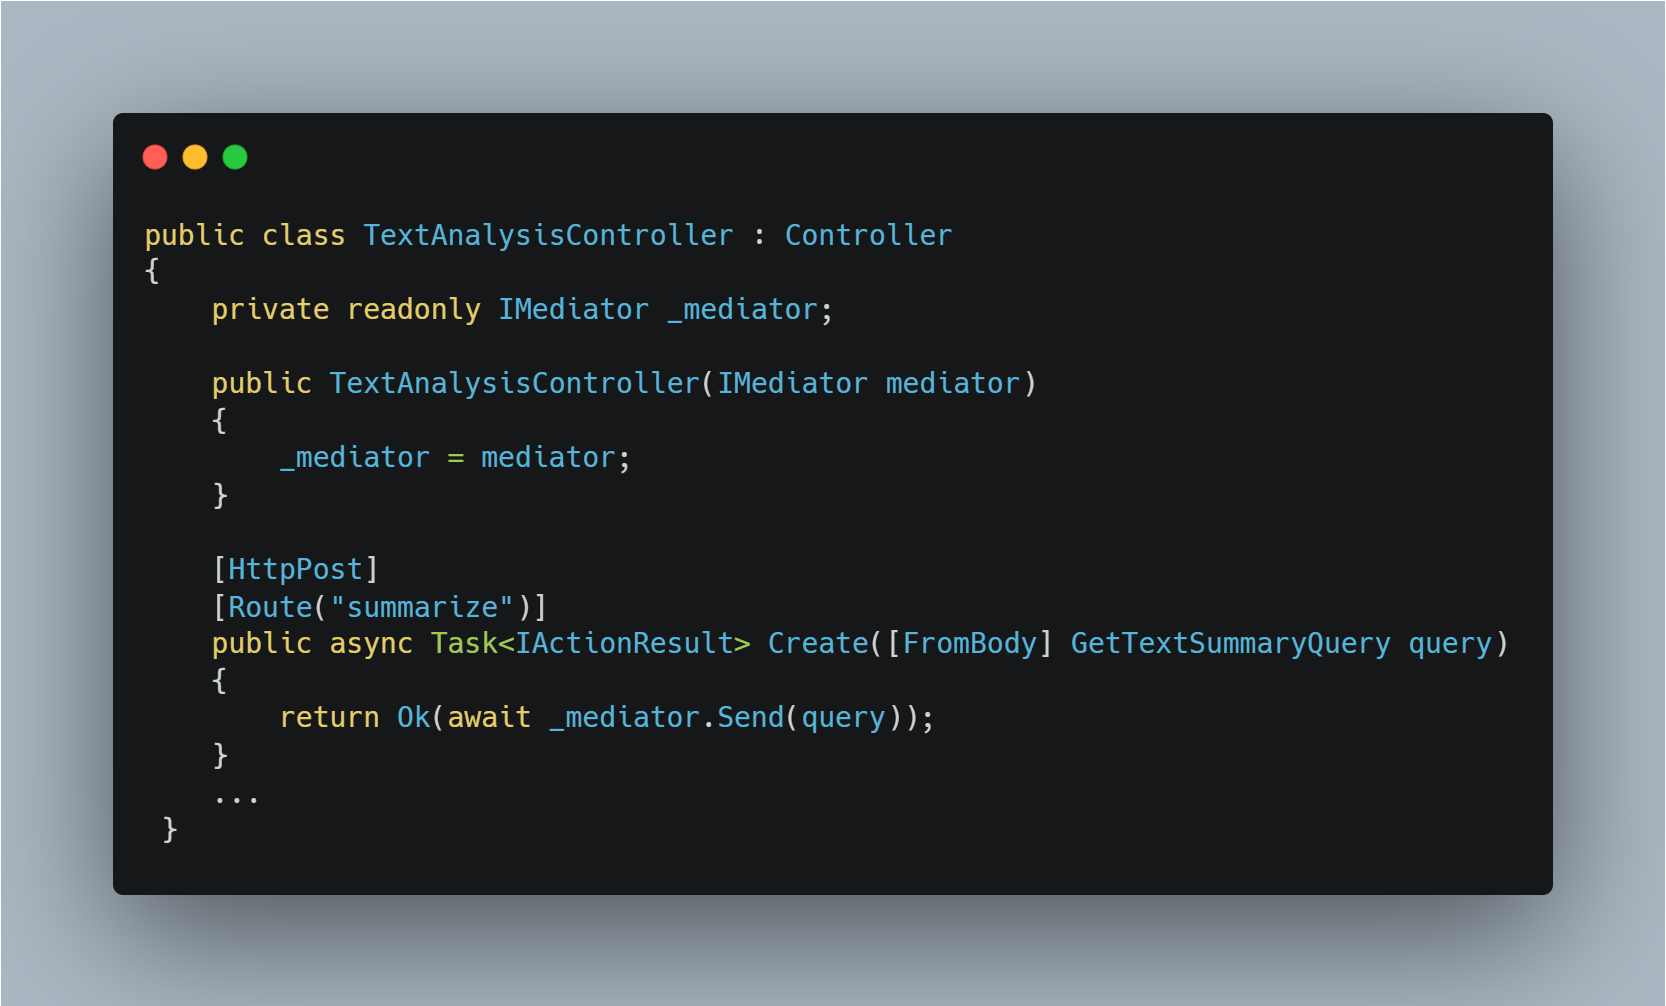
\includegraphics[width=150mm]{figs/controllerExample.png}
	\caption{Exemplu de controller cu Mediator}
	\label{fig:controllerExample}
\end{figure}

\section{Structura modulului de frontend}
În figura \ref{fig:frontendDiagram} este reprezentată diagrama modulului de backend.
\begin{figure}[H]
	\centering
	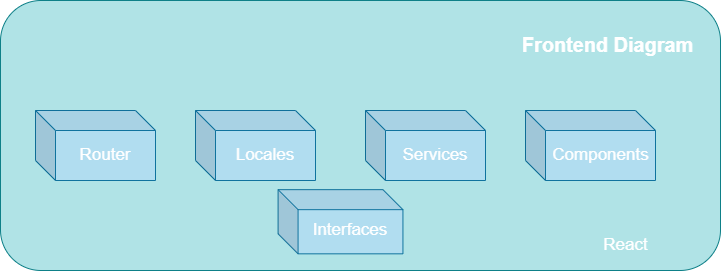
\includegraphics[width=150mm]{figs/frontendDiagram.png}
	\caption{Diagrama modulului de frontend}
	\label{fig:frontendDiagram}
\end{figure}

Diagrama pachetelor din acest modul poate fi văzută în figura \ref{fig:packageFE}.
\begin{figure}[h]
	\centering
	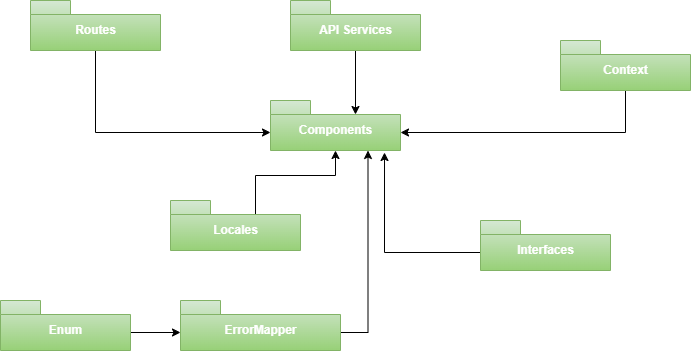
\includegraphics[width=150mm]{figs/packageFE.png}
	\caption{Diagrama pachetelor din modulul de frontend}
	\label{fig:packageFE}
\end{figure}

\subsubsection{Routes}

În modulul de frontend, componenta de Router se ocupă de rutare. \\ În general, o rută randează o pagină pentru un anumit URL.
În aplicație, pentru securitatea utilizatorului, au fost create rute publice și private. \\

Rutele publice reprezintă rutele pe care utilizatorul le poate accesa atunci când nu este autentificat, adică poate accesa paginile de Creare cont nou și de Logare în aplicație.\\

Pentru un utilizator neautentificat, orice încercare de a modifica forțat URL-ul și a accesa o rută privată, se rezumă la o redirecționare la o pagină cu rută publică.
Pentru rutele private, utilizatorul trebuie să aibă un cont creat și să fie logat. 
Pentru un utilizator autentificat, orice încercare de a modifica forțat URL-ul și accesa o rută publică, se rezumă la o redirecționare la pagina de Dashboard.\\

Pentru a putea gestiona global starea și pentru a obține statusul utilizatorului, dacă acesta este logat sau nu, se folosește un Context \ref{fig:reactContext}~\cite{ReactContext}.
\begin{figure}[h]
	\centering
	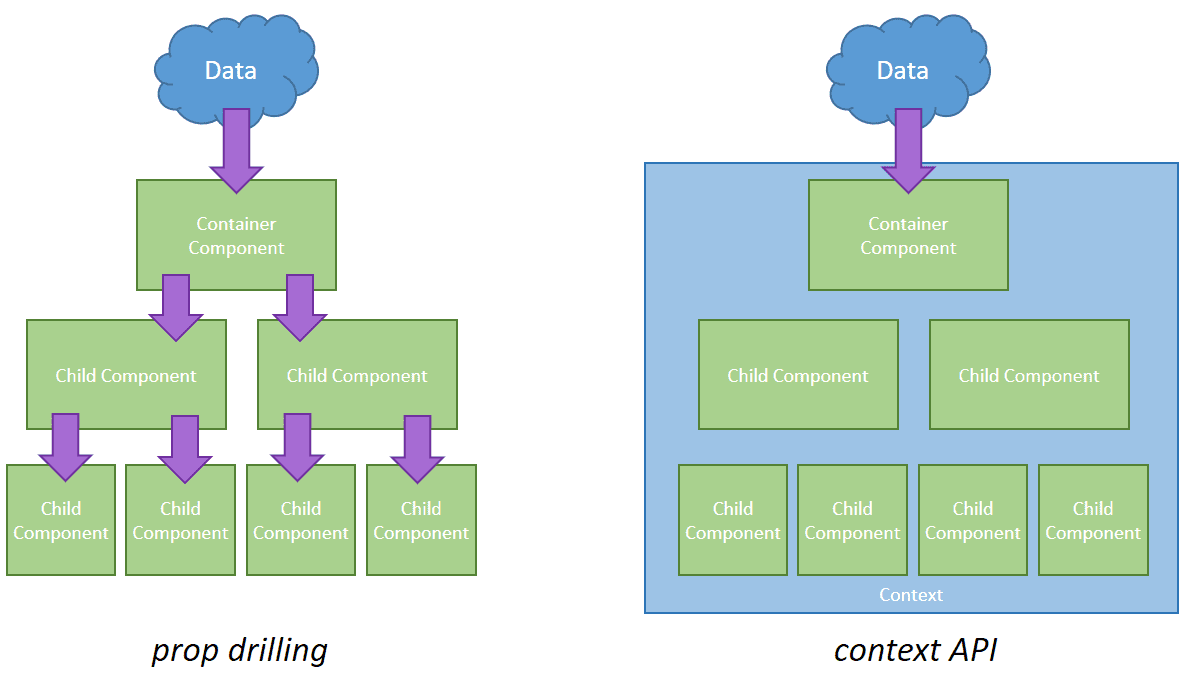
\includegraphics[width=150mm]{figs/reactContext.png}
	\caption{Contextul în React}
	\label{fig:reactContext}
\end{figure}

\subsubsection{Locales}
Internaționalizarea este implementarea unei aplicații astfel încât aceasta să fie disponibilă pentru utilizatori, indiferent de regiune.\\
Acest obiectiv a fost atins folosind i18n. Au fost create traduceri pentru toate textele din aplicație, fiind disponibile atunci când utilizatorul folosește switch-ul de limbă. 
Preferința utilizatorului va rămâne salvată, astfel încât atunci când va închide browserul și va reveni, va găsi aplicația în aceeași limbă.
\\

În fișierul index.ts din figura \ref{fig:i18nInstance}, trebuie asigurat faptul că librăria i18n este instalată și importurile sunt făcute pentru a beneficia de funționalitate.\\
Cu ajutorul funcției {\it use(...)} se pasează pluginul de i18n, apoi este inițializat cu resursele, care sunt fișierele de traduceri. În această aplicație, traducerile sunt pentru limba Engleză și limba Română.\\

{\it lng} este limba de început, dacă în localStorage există valoare pentru atributul 'language', atunci va fi folosit, altfel va fi folosită limba engleză. \\

Proprietatea de interpolare se referă la integrarea dinamică a valorilor în traduceri, iar opțiunea de escapeValue se referă la escaparea valorilor pentru a evita atacurile de tip XSS (Cross Site Scripting).
Acest tip de atac apare atunci când scripturi malițioase sunt injectate în paginile web, vizând alți utilizatori ai aplicației.\\

Atributul de keySeparator se folosește pentru a separa cheile cu un caracter definit în această configurare. Pentru că traducerile sunt JSON cu format key-value, este recomandat să fie setat pe false.

\begin{figure}[h]
	\centering
	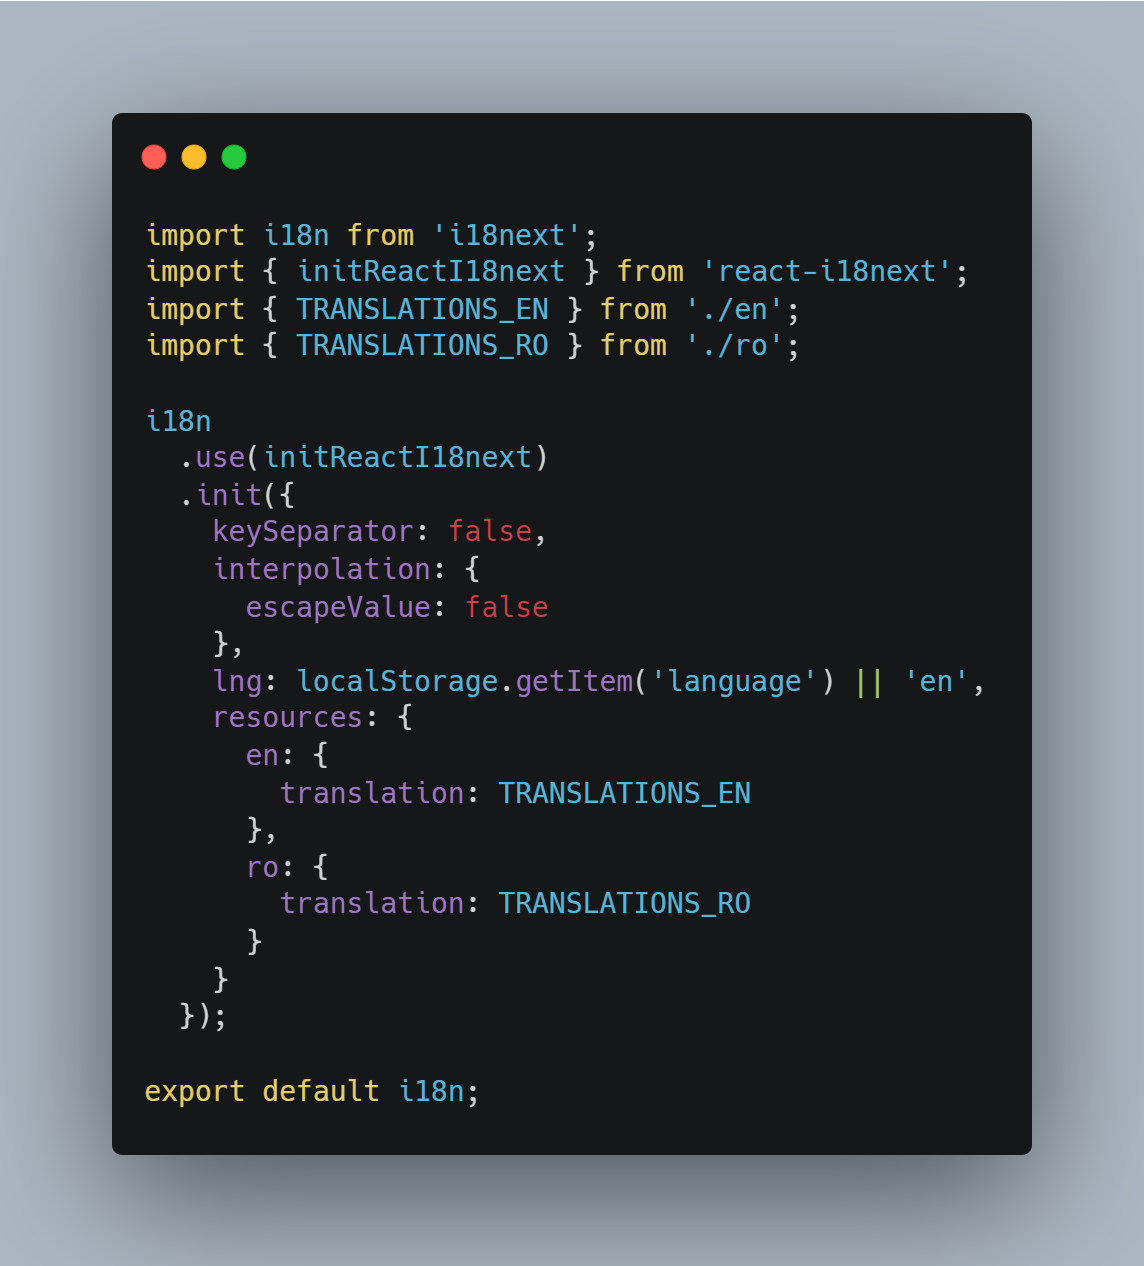
\includegraphics[width=150mm, height=150mm]{figs/i18nInstance.png}
	\caption{Configurare i18n}
	\label{fig:i18nInstance}
\end{figure}

\subsubsection{Services}
Pentru partea de servicii API și comunicare cu serverul, Axios este o librărie care ajută la creare request-urilor HTTP la endpoint-urile REST pentru a executa operații de stocare, citire, actualizare, ștergere (CRUD).\\
Folosind Axios cu un URL și, opțional un body, se obține un Promise care returnează un răspuns, după cum se poate vedea în figura \ref{fig:axiosPromise}.
\begin{figure}[h]
	\centering
	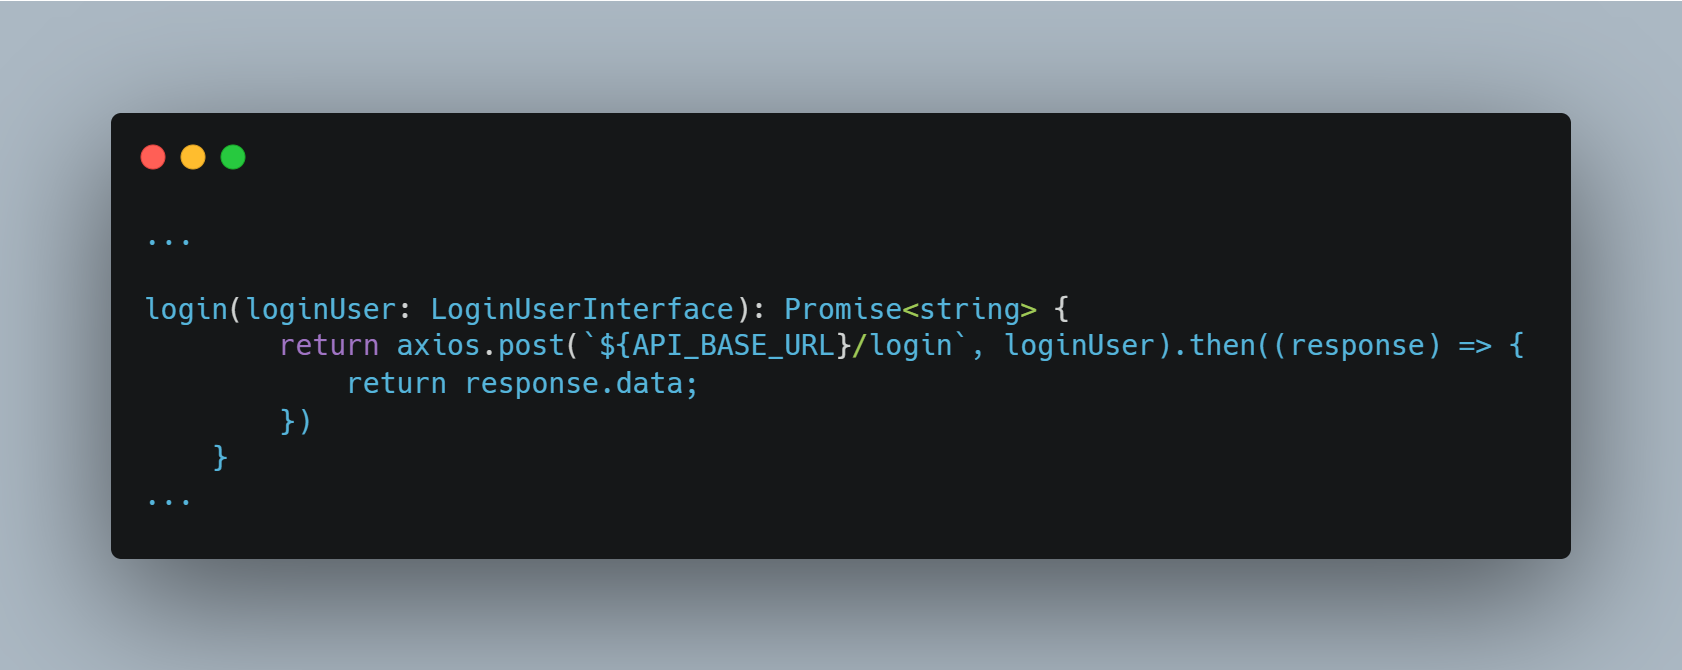
\includegraphics[width=150mm]{figs/axiosPromise.png}
	\caption{Structură request Axios}
	\label{fig:axiosPromise}
\end{figure}

\subsubsection{Components}
Componentele folosite în aplicație sunt din librările Ant Design, iar graficele sunt din librăria recharts. Pentru customizarea ambelor componente s-a folosit styled-components, cu o metodă de a aplica stilul numită CSS-in-JS. \\
Un exemplu de aplicare a stilului pe o componentă se poate vedea în figura \ref{fig:cssStyle}, iar rezultatul final în figura \ref{fig:notFoundPage}.
Se crează o componentă reutilizabilă numită Button404 (această componentă apare în pagina Not Fount) și moștenește stilul inițial al componentei din AntD prin {\it styled(Button)}. \\

\noindent Customizare componentei începe acum, când este setată o culoare de background pentru buton iar scrisul trebuie să fie alb (color: white). Se setează dimensiunilor butonului și un border-radius de 12 pixeli pentru a rotunji marginile butonului. 
\begin{figure}[h]
	\centering
	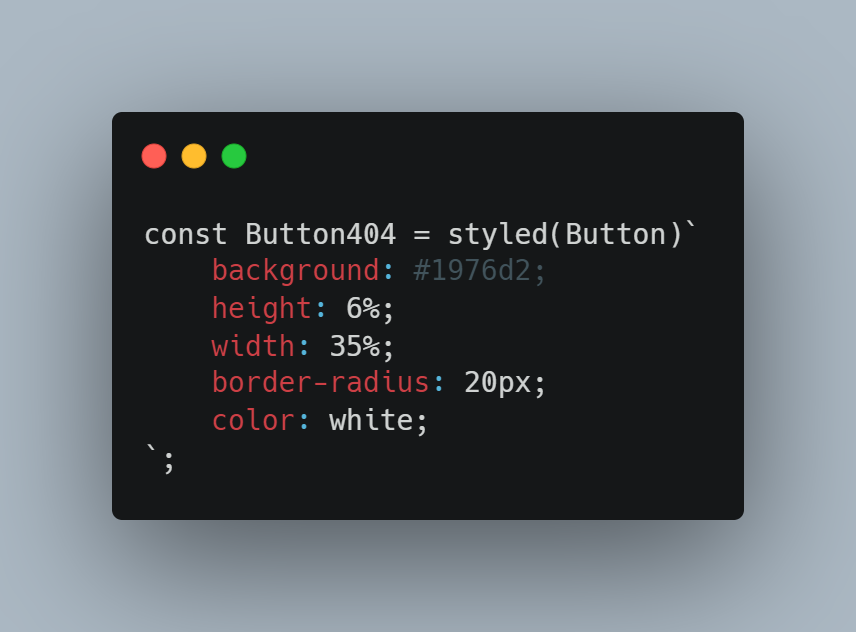
\includegraphics[width=100mm]{figs/cssStyle.png}
	\caption{Mod de aplicare a stilului folosind styled-components pe o componentă AntD}
	\label{fig:cssStyle}
\end{figure}

\newpage

\begin{figure}[h]
	\centering
	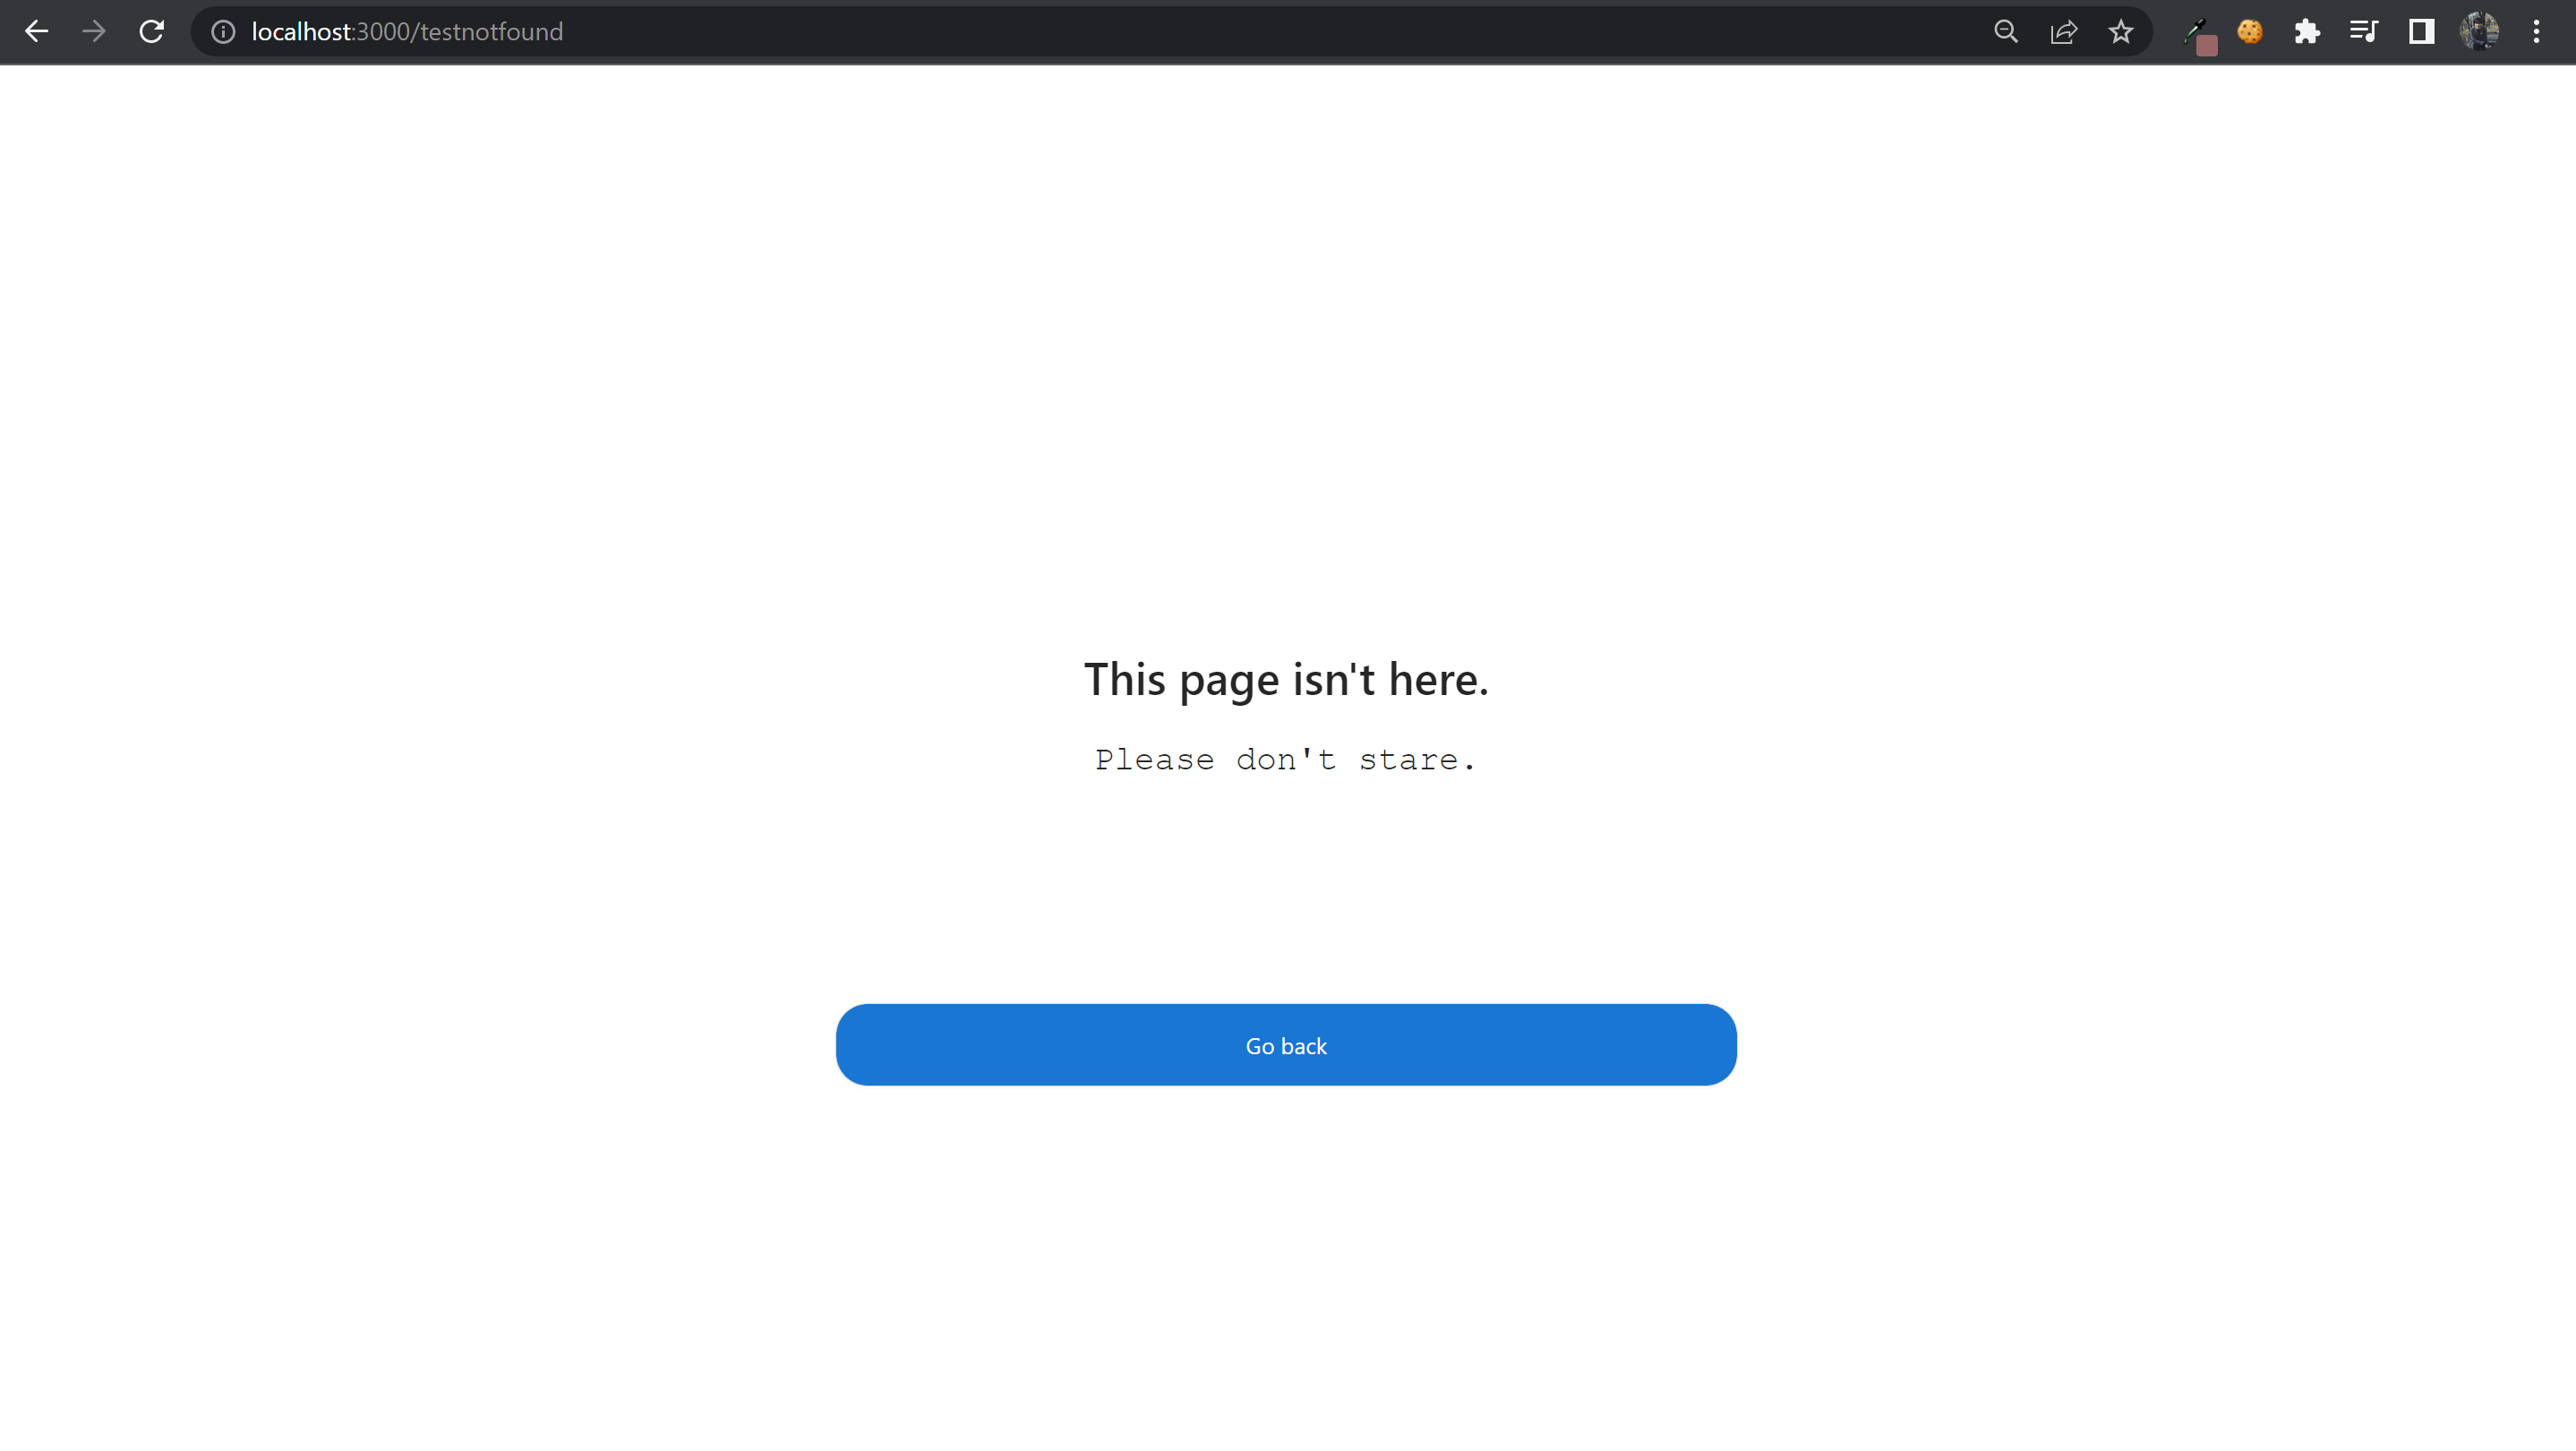
\includegraphics[width=100mm]{figs/notFoundPage.png}
	\caption{Stilul aplicat pe butonul din pagina de Not Found}
	\label{fig:notFoundPage}
\end{figure}

\begin{figure}[h]
	\centering
	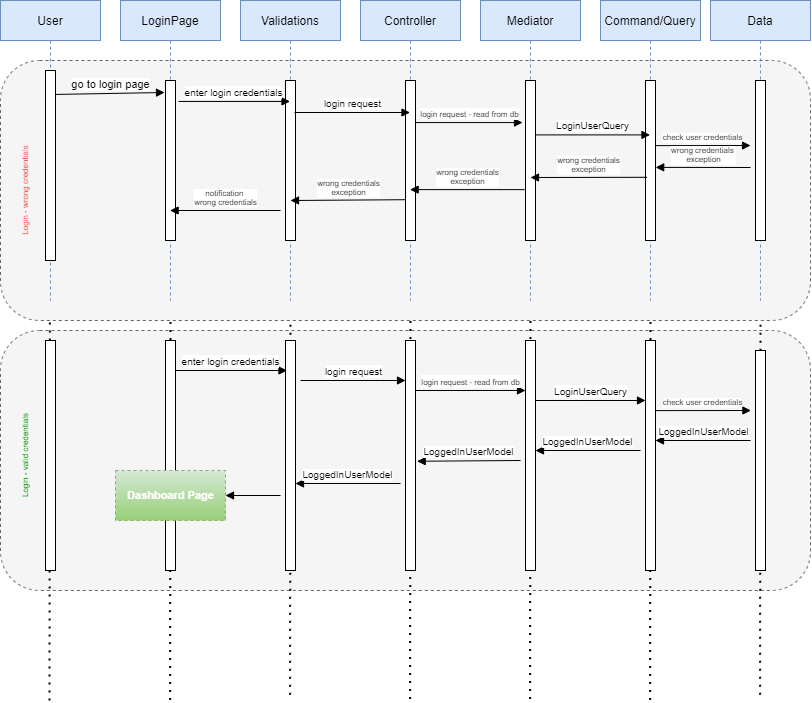
\includegraphics[width=150mm]{figs/sequnce.png}
	\caption{Diagramă de secvență pentru logarea în aplicație}
	\label{fig:sequnce}
\end{figure} 

\ \\ 
\section{Analizarea textului}
Aplicația realizează inferența pentru analiza sentimentelor din textele analizate, pentru sumarizarea textului și pentru extragerea cuvintelor cheie.\\
Hugging Face Inference API este accesat printr-un request HTTP, incluzând în body-ul requestului textul de la utilizator.\\

Cuvintele cheie sau expresiile sunt extrase din textul original și sunt evidențiate atât în partea de text original, cât și în partea de text sumarizat din pagina de Dashboard din frontend.\\
După extragerea cuvintelor cheie, acestea sunt salvate în baza de date, de unde se fac următoarele procesări, în funcție de inputul utilizatorului: \\

Pentru generarea graficului cu cele mai populare subiecte dintr-o anumită perioadă, se transmite o cerere cu perioada la server.\\
Mai departe, serverul caută în baza de date înregistrarile care corespund perioadei căutate și le contorizează în funcție de nume.
La final, rezultatul transmis este o listă de 10 elemente care conține obiecte constituite din numele cuvintelor și numărul de apariții, în acest fel fiind generat graficul de trending.\\

Pentru generarea graficului de evoluție al unui cuvânt cheie sau expresii, inputul trebuie să conțină perioada și cuvântul/cuvintele cautate.
Se face o căutare a înregistrărilor din baza de date care corespund perioadei căutate și al cărui nume corespunde cu inputul utilizatorului.\\
Înregistrarările care corespund căutării sunt ordonate apoi după data în care au fost salvate.
Rezultatul acestui filtru este o listă care conține obiecte constituite din ziua înregistrarii și numărul de apariții din acea zi.\\

WordCloud-ul este o colecție de cuvinte sau expresii de diferite mărimi. \\
Pentru generarea acestuia, la fel ca pentru graficul de trending, este nevoie de numărul de apariții pentru fiecare termen existent
în înregistrări. Diferența dintre cele două este că graficul de trending care este limitat la 10 elemente.\\
În funcție de numărul de înregistrări pentru un anumit termen, dimensiunea acestuia o sa varieze atunci când este afișat.
